%\subsection*{How to find the Higgs boson?} 
%\begin{frame}
\frametitle{Using histograms}

\manip Find a discriminating variable:
\submanip for uncorrelated \tau\ pairs, it's random
\submanip for \tau\ pairs coming from a particle (Higgs?), not random.

\manip For one \tau\ pair only, impossible to say!

\manip With many events, a difference may show up.
\end{frame}

\begin{frame}
\frametitle{The rabbit analogy}
\beamercite{Higgs_discovery_explained_video_3}

\manip White rabbit that once lived in a casino.
\submanip The rabbit loved watching people playing dices.
\submanip He was happy when the result of dice was 4.
\submanip So when he sees a dice, he turns it so that the result is 4.
\submanip But this rabbit is very shy and nobody has seen him since the casino closure.
\submanip The only way to know if he's here is to throw a dice and come back to see the result.
\submanip If the rabbit has been here, the dice will show a 4!
\end{frame}

\begin{frame}
\frametitle{The rabbit analogy}
\beamercite{Higgs_discovery_explained_video_3}

\manip Dice results:
4\pause,
2\pause,
4,
1,
3,
2,
5,
1,
1,
6...
\end{frame}

\begin{frame}
\frametitle{The rabbit analogy}
\beamercite{Higgs_discovery_explained_video_3}
\begin{center}
\begin{minipage}[c]{.29\textwidth}
On \num{100} days $\rightarrow$
\end{minipage}
\begin{minipage}[c]{.4\textwidth}
\vspace{-\baselineskip}
\includegraphics[height=\graphh, width=\graphw,keepaspectratio]{/home/torterotot/Documents/PhD-Thesis/plots_and_images/my_plots/inspired_from_Higgs_discovery_explained_video_3/1-only_data_100-pyplot.tex}
\end{minipage}
\begin{minipage}[c]{.29\textwidth}
Not really conclusive...
\end{minipage}
\end{center}
\end{frame}

\begin{frame}
\frametitle{The rabbit analogy}
\addtocounter{framenumber}{-1}
\beamercite{Higgs_discovery_explained_video_3}
\begin{center}
\begin{minipage}[c]{.29\textwidth}
On \num{100} days $\rightarrow$
\end{minipage}
\begin{minipage}[c]{.4\textwidth}
\vspace{-\baselineskip}
\includegraphics[height=\graphh, width=\graphw,keepaspectratio]{/home/torterotot/Documents/PhD-Thesis/plots_and_images/my_plots/inspired_from_Higgs_discovery_explained_video_3/2-data_and_bg_estim_100-pyplot.tex}
\end{minipage}
\begin{minipage}[c]{.29\textwidth}
Comparing with predictions!
\end{minipage}
\end{center}
\end{frame}

\begin{frame}
\frametitle{The rabbit analogy}
\addtocounter{framenumber}{-1}
\beamercite{Higgs_discovery_explained_video_3}
\begin{center}
\begin{minipage}[c]{.29\textwidth}
On \num{100} days $\rightarrow$
\end{minipage}
\begin{minipage}[c]{.4\textwidth}
\vspace{-\baselineskip}
\includegraphics[height=\graphh, width=\graphw,keepaspectratio]{/home/torterotot/Documents/PhD-Thesis/plots_and_images/my_plots/inspired_from_Higgs_discovery_explained_video_3/3-data_and_bg_estim_ratio_100-pyplot.tex}
\end{minipage}
\begin{minipage}[c]{.29\textwidth}
Also add ratio plot:\\
observed / predictions
\end{minipage}
\end{center}
\end{frame}

\begin{frame}
\frametitle{The rabbit analogy}
\addtocounter{framenumber}{-1}
\beamercite{Higgs_discovery_explained_video_3}
\begin{center}
\begin{minipage}[c]{.29\textwidth}
On \num{100} days $\rightarrow$
\end{minipage}
\begin{minipage}[c]{.4\textwidth}
\vspace{-\baselineskip}
\includegraphics[height=\graphh, width=\graphw,keepaspectratio]{/home/torterotot/Documents/PhD-Thesis/plots_and_images/my_plots/inspired_from_Higgs_discovery_explained_video_3/4-up_to_100-pyplot.tex}
\end{minipage}
\begin{minipage}[c]{.29\textwidth}
Fill up with more data!
\end{minipage}
\end{center}
\end{frame}

%\begin{frame}
%\frametitle{The rabbit analogy}
%\addtocounter{framenumber}{-1}
%\transwipe[direction=90]
%\beamercite{Higgs_discovery_explained_video_3}
%\begin{center}
%\begin{minipage}[c]{.29\textwidth}
%On \num{500} days $\rightarrow$
%\end{minipage}
%\begin{minipage}[c]{.4\textwidth}
%\vspace{-\baselineskip}
%\includegraphics[height=\graphh, width=\graphw,keepaspectratio]{/home/torterotot/Documents/PhD-Thesis/plots_and_images/my_plots/inspired_from_Higgs_discovery_explained_video_3/5-up_to_500-pyplot.tex}
%\end{minipage}
%\begin{minipage}[c]{.29\textwidth}
%Fill up with more data!
%\end{minipage}
%\end{center}
%\end{frame}

\begin{frame}
\frametitle{The rabbit analogy}
\addtocounter{framenumber}{-1}
\transwipe[direction=90]
\beamercite{Higgs_discovery_explained_video_3}
\begin{center}
\begin{minipage}[c]{.29\textwidth}
On \num{1000} days $\rightarrow$
\end{minipage}
\begin{minipage}[c]{.4\textwidth}
\vspace{-\baselineskip}
\includegraphics[height=\graphh, width=\graphw,keepaspectratio]{/home/torterotot/Documents/PhD-Thesis/plots_and_images/my_plots/inspired_from_Higgs_discovery_explained_video_3/6-up_to_1000-pyplot.tex}
\end{minipage}
\begin{minipage}[c]{.29\textwidth}
Fill up with more data!
\end{minipage}
\end{center}
\end{frame}

%\begin{frame}
%\frametitle{The rabbit analogy}
%\addtocounter{framenumber}{-1}
%\transwipe[direction=90]
%\transduration{0}
%\beamercite{Higgs_discovery_explained_video_3}
%\begin{center}
%\begin{minipage}[c]{.29\textwidth}
%On \num{1500} days $\rightarrow$
%\end{minipage}
%\begin{minipage}[c]{.4\textwidth}
%\vspace{-\baselineskip}
%\includegraphics[height=\graphh, width=\graphw,keepaspectratio]{/home/torterotot/Documents/PhD-Thesis/plots_and_images/my_plots/inspired_from_Higgs_discovery_explained_video_3/7-up_to_1500-pyplot.tex}
%\end{minipage}
%\begin{minipage}[c]{.29\textwidth}
%Fill up with more data!
%\end{minipage}
%\end{center}
%\end{frame}

\begin{frame}
\frametitle{The rabbit analogy}
\addtocounter{framenumber}{-1}
\transwipe[direction=90]
\transduration{0}
\beamercite{Higgs_discovery_explained_video_3}
\begin{center}
\begin{minipage}[c]{.29\textwidth}
On \num{2000} days $\rightarrow$
\end{minipage}
\begin{minipage}[c]{.4\textwidth}
\vspace{-\baselineskip}
\includegraphics[height=\graphh, width=\graphw,keepaspectratio]{/home/torterotot/Documents/PhD-Thesis/plots_and_images/my_plots/inspired_from_Higgs_discovery_explained_video_3/8-up_to_2000-pyplot.tex}
\end{minipage}
\begin{minipage}[c]{.29\textwidth}
Fill up with more data!
\end{minipage}
\end{center}
\end{frame}

%\begin{frame}
%\frametitle{The rabbit analogy}
%\addtocounter{framenumber}{-1}
%\transwipe[direction=90]
%\transduration{0}
%\beamercite{Higgs_discovery_explained_video_3}
%\begin{center}
%\begin{minipage}[c]{.29\textwidth}
%On \num{2500} days $\rightarrow$
%\end{minipage}
%\begin{minipage}[c]{.4\textwidth}
%\vspace{-\baselineskip}
%\includegraphics[height=\graphh, width=\graphw,keepaspectratio]{/home/torterotot/Documents/PhD-Thesis/plots_and_images/my_plots/inspired_from_Higgs_discovery_explained_video_3/9-up_to_2500-pyplot.tex}
%\end{minipage}
%\begin{minipage}[c]{.29\textwidth}
%Fill up with more data!
%\end{minipage}
%\end{center}
%\end{frame}

\begin{frame}
\frametitle{The rabbit analogy}
\addtocounter{framenumber}{-1}
\transwipe[direction=90]
\transduration{0}
\beamercite{Higgs_discovery_explained_video_3}
\begin{center}
\begin{minipage}[c]{.29\textwidth}
On \num{3000} days $\rightarrow$
\end{minipage}
\begin{minipage}[c]{.4\textwidth}
\vspace{-\baselineskip}
\includegraphics[height=\graphh, width=\graphw,keepaspectratio]{/home/torterotot/Documents/PhD-Thesis/plots_and_images/my_plots/inspired_from_Higgs_discovery_explained_video_3/10-up_to_3000-pyplot.tex}
\end{minipage}
\begin{minipage}[c]{.29\textwidth}
Fill up with more data!
\end{minipage}
\end{center}
\end{frame}

%\begin{frame}
%\frametitle{The rabbit analogy}
%\addtocounter{framenumber}{-1}
%\transwipe[direction=90]
%\transduration{0}
%\beamercite{Higgs_discovery_explained_video_3}
%\begin{center}
%\begin{minipage}[c]{.29\textwidth}
%On \num{3500} days $\rightarrow$
%\end{minipage}
%\begin{minipage}[c]{.4\textwidth}
%\vspace{-\baselineskip}
%\includegraphics[height=\graphh, width=\graphw,keepaspectratio]{/home/torterotot/Documents/PhD-Thesis/plots_and_images/my_plots/inspired_from_Higgs_discovery_explained_video_3/11-up_to_3500-pyplot.tex}
%\end{minipage}
%\begin{minipage}[c]{.29\textwidth}
%Fill up with more data!
%\end{minipage}
%\end{center}
%\end{frame}

\begin{frame}
\frametitle{The rabbit analogy}
\addtocounter{framenumber}{-1}
\transwipe[direction=90]
\transduration{0}
\beamercite{Higgs_discovery_explained_video_3}
\begin{center}
\begin{minipage}[c]{.29\textwidth}
On \num{4000} days $\rightarrow$
\end{minipage}
\begin{minipage}[c]{.4\textwidth}
\vspace{-\baselineskip}
\includegraphics[height=\graphh, width=\graphw,keepaspectratio]{/home/torterotot/Documents/PhD-Thesis/plots_and_images/my_plots/inspired_from_Higgs_discovery_explained_video_3/12-up_to_4000-pyplot.tex}
\end{minipage}
\begin{minipage}[c]{.29\textwidth}
Fill up with more data!
\end{minipage}
\end{center}
\end{frame}

%\begin{frame}
%\frametitle{The rabbit analogy}
%\addtocounter{framenumber}{-1}
%\transwipe[direction=90]
%\transduration{0}
%\beamercite{Higgs_discovery_explained_video_3}
%\begin{center}
%\begin{minipage}[c]{.29\textwidth}
%On \num{4500} days $\rightarrow$
%\end{minipage}
%\begin{minipage}[c]{.4\textwidth}
%\vspace{-\baselineskip}
%\includegraphics[height=\graphh, width=\graphw,keepaspectratio]{/home/torterotot/Documents/PhD-Thesis/plots_and_images/my_plots/inspired_from_Higgs_discovery_explained_video_3/13-up_to_4500-pyplot.tex}
%\end{minipage}
%\begin{minipage}[c]{.29\textwidth}
%Fill up with more data!
%\end{minipage}
%\end{center}
%\end{frame}

\begin{frame}
\frametitle{The rabbit analogy}
\addtocounter{framenumber}{-1}
\transwipe[direction=90]
\transduration{0}
\beamercite{Higgs_discovery_explained_video_3}
\begin{center}
\begin{minipage}[c]{.29\textwidth}
On \num{5000} days $\rightarrow$
\end{minipage}
\begin{minipage}[c]{.4\textwidth}
\vspace{-\baselineskip}
\includegraphics[height=\graphh, width=\graphw,keepaspectratio]{/home/torterotot/Documents/PhD-Thesis/plots_and_images/my_plots/inspired_from_Higgs_discovery_explained_video_3/14-up_to_5000-pyplot.tex}
\end{minipage}
\begin{minipage}[c]{.29\textwidth}
Fill up with more data!
\end{minipage}
\end{center}
\end{frame}

%\begin{frame}
%\frametitle{The rabbit analogy}
%\addtocounter{framenumber}{-1}
%\transwipe[direction=90]
%\transduration{0}
%\beamercite{Higgs_discovery_explained_video_3}
%\begin{center}
%\begin{minipage}[c]{.29\textwidth}
%On \num{5500} days $\rightarrow$
%\end{minipage}
%\begin{minipage}[c]{.4\textwidth}
%\vspace{-\baselineskip}
%\includegraphics[height=\graphh, width=\graphw,keepaspectratio]{/home/torterotot/Documents/PhD-Thesis/plots_and_images/my_plots/inspired_from_Higgs_discovery_explained_video_3/15-up_to_5500-pyplot.tex}
%\end{minipage}
%\begin{minipage}[c]{.29\textwidth}
%Fill up with more data!
%\end{minipage}
%\end{center}
%\end{frame}

\begin{frame}
\frametitle{The rabbit analogy}
\addtocounter{framenumber}{-1}
\transwipe[direction=90]
\transduration{0}
\beamercite{Higgs_discovery_explained_video_3}
\begin{center}
\begin{minipage}[c]{.29\textwidth}
On \num{6000} days $\rightarrow$
\end{minipage}
\begin{minipage}[c]{.4\textwidth}
\vspace{-\baselineskip}
\includegraphics[height=\graphh, width=\graphw,keepaspectratio]{/home/torterotot/Documents/PhD-Thesis/plots_and_images/my_plots/inspired_from_Higgs_discovery_explained_video_3/16-up_to_6000-pyplot.tex}
\end{minipage}
\begin{minipage}[c]{.29\textwidth}
Fill up with more data!
\end{minipage}
\end{center}
\end{frame}

%\begin{frame}
%\frametitle{The rabbit analogy}
%\addtocounter{framenumber}{-1}
%\transwipe[direction=90]
%\transduration{0}
%\beamercite{Higgs_discovery_explained_video_3}
%\begin{center}
%\begin{minipage}[c]{.29\textwidth}
%On \num{6500} days $\rightarrow$
%\end{minipage}
%\begin{minipage}[c]{.4\textwidth}
%\vspace{-\baselineskip}
%\includegraphics[height=\graphh, width=\graphw,keepaspectratio]{/home/torterotot/Documents/PhD-Thesis/plots_and_images/my_plots/inspired_from_Higgs_discovery_explained_video_3/17-up_to_6500-pyplot.tex}
%\end{minipage}
%\begin{minipage}[c]{.29\textwidth}
%Fill up with more data!
%\end{minipage}
%\end{center}
%\end{frame}

\begin{frame}
\frametitle{The rabbit analogy}
\addtocounter{framenumber}{-1}
\transwipe[direction=90]
\transduration{0}
\beamercite{Higgs_discovery_explained_video_3}
\begin{center}
\begin{minipage}[c]{.29\textwidth}
On \num{7000} days $\rightarrow$
\end{minipage}
\begin{minipage}[c]{.4\textwidth}
\vspace{-\baselineskip}
\includegraphics[height=\graphh, width=\graphw,keepaspectratio]{/home/torterotot/Documents/PhD-Thesis/plots_and_images/my_plots/inspired_from_Higgs_discovery_explained_video_3/18-up_to_7000-pyplot.tex}
\end{minipage}
\begin{minipage}[c]{.29\textwidth}
Fill up with more data!
\end{minipage}
\end{center}
\end{frame}

%\begin{frame}
%\frametitle{The rabbit analogy}
%\addtocounter{framenumber}{-1}
%\transwipe[direction=90]
%\transduration{0}
%\beamercite{Higgs_discovery_explained_video_3}
%\begin{center}
%\begin{minipage}[c]{.29\textwidth}
%On \num{7500} days $\rightarrow$
%\end{minipage}
%\begin{minipage}[c]{.4\textwidth}
%\vspace{-\baselineskip}
%\includegraphics[height=\graphh, width=\graphw,keepaspectratio]{/home/torterotot/Documents/PhD-Thesis/plots_and_images/my_plots/inspired_from_Higgs_discovery_explained_video_3/19-up_to_7500-pyplot.tex}
%\end{minipage}
%\begin{minipage}[c]{.29\textwidth}
%Fill up with more data!
%\end{minipage}
%\end{center}
%\end{frame}

\begin{frame}
\frametitle{The rabbit analogy}
\addtocounter{framenumber}{-1}
\transwipe[direction=90]
\transduration{0}
\beamercite{Higgs_discovery_explained_video_3}
\begin{center}
\begin{minipage}[c]{.29\textwidth}
On \num{8000} days $\rightarrow$
\end{minipage}
\begin{minipage}[c]{.4\textwidth}
\vspace{-\baselineskip}
\includegraphics[height=\graphh, width=\graphw,keepaspectratio]{/home/torterotot/Documents/PhD-Thesis/plots_and_images/my_plots/inspired_from_Higgs_discovery_explained_video_3/20-up_to_8000-pyplot.tex}
\end{minipage}
\begin{minipage}[c]{.29\textwidth}
Fill up with more data!
\end{minipage}
\end{center}
\end{frame}

%\begin{frame}
%\frametitle{The rabbit analogy}
%\addtocounter{framenumber}{-1}
%\transwipe[direction=90]
%\transduration{0}
%\beamercite{Higgs_discovery_explained_video_3}
%\begin{center}
%\begin{minipage}[c]{.29\textwidth}
%On \num{8500} days $\rightarrow$
%\end{minipage}
%\begin{minipage}[c]{.4\textwidth}
%\vspace{-\baselineskip}
%\includegraphics[height=\graphh, width=\graphw,keepaspectratio]{/home/torterotot/Documents/PhD-Thesis/plots_and_images/my_plots/inspired_from_Higgs_discovery_explained_video_3/21-up_to_8500-pyplot.tex}
%\end{minipage}
%\begin{minipage}[c]{.29\textwidth}
%Fill up with more data!
%\end{minipage}
%\end{center}
%\end{frame}

\begin{frame}
\frametitle{The rabbit analogy}
\addtocounter{framenumber}{-1}
\transwipe[direction=90]
\transduration{0}
\beamercite{Higgs_discovery_explained_video_3}
\begin{center}
\begin{minipage}[c]{.29\textwidth}
On \num{9000} days $\rightarrow$
\end{minipage}
\begin{minipage}[c]{.4\textwidth}
\vspace{-\baselineskip}
\includegraphics[height=\graphh, width=\graphw,keepaspectratio]{/home/torterotot/Documents/PhD-Thesis/plots_and_images/my_plots/inspired_from_Higgs_discovery_explained_video_3/22-up_to_9000-pyplot.tex}
\end{minipage}
\begin{minipage}[c]{.29\textwidth}
Fill up with more data!
\end{minipage}
\end{center}
\end{frame}

%\begin{frame}
%\frametitle{The rabbit analogy}
%\addtocounter{framenumber}{-1}
%\transwipe[direction=90]
%\transduration{0}
%\beamercite{Higgs_discovery_explained_video_3}
%\begin{center}
%\begin{minipage}[c]{.29\textwidth}
%On \num{9500} days $\rightarrow$
%\end{minipage}
%\begin{minipage}[c]{.4\textwidth}
%\vspace{-\baselineskip}
%\includegraphics[height=\graphh, width=\graphw,keepaspectratio]{/home/torterotot/Documents/PhD-Thesis/plots_and_images/my_plots/inspired_from_Higgs_discovery_explained_video_3/23-up_to_9500-pyplot.tex}
%\end{minipage}
%\begin{minipage}[c]{.29\textwidth}
%Fill up with more data!
%\end{minipage}
%\end{center}
%\end{frame}

\begin{frame}
\frametitle{The rabbit analogy}
\addtocounter{framenumber}{-1}
\transwipe[direction=90]
\beamercite{Higgs_discovery_explained_video_3}
\begin{center}
\begin{minipage}[c]{.29\textwidth}
On \num{10000} days $\rightarrow$
\end{minipage}
\begin{minipage}[c]{.4\textwidth}
\vspace{-\baselineskip}
\includegraphics[height=\graphh, width=\graphw,keepaspectratio]{/home/torterotot/Documents/PhD-Thesis/plots_and_images/my_plots/inspired_from_Higgs_discovery_explained_video_3/24-up_to_10000-pyplot.tex}
\end{minipage}
\begin{minipage}[c]{.29\textwidth}
Fill up with more data!
\end{minipage}
\end{center}
\end{frame}

\begin{frame}
\frametitle{The rabbit analogy}
\addtocounter{framenumber}{-1}
\transdissolve
\beamercite{Higgs_discovery_explained_video_3}
\begin{center}
\begin{minipage}[c]{.29\textwidth}
On \num{10000} days $\rightarrow$
\end{minipage}
\begin{minipage}[c]{.4\textwidth}
\vspace{-\baselineskip}
\includegraphics[height=\graphh, width=\graphw,keepaspectratio]{/home/torterotot/Documents/PhD-Thesis/plots_and_images/my_plots/inspired_from_Higgs_discovery_explained_video_3/25-up_to_10000_SR-pyplot.tex}
\end{minipage}
\begin{minipage}[c]{.29\textwidth}
In red, hypothesis of the rabbit with 3 as preffered result\\
(instead of 4!), with a probability to show up of \SI{5}{\%}.
\end{minipage}
\end{center}
\end{frame}


%\subsection*{Events selections}
%\begin{frame}
\frametitle{Signal region (SR) for semi-leptonic channels ($\ell\tauh$)}

\begin{block}{Particles identification}
\begin{multicols}{2}
\begin{itemize}
\item $\ell$ ID:
\begin{itemize}
\item \mu: medium (eff. \SI{99.5}{\%})
\item \ele: tight (eff. \SI{80}{\%})
\end{itemize}
\item \tauh\ ID:
\begin{itemize}
\item vs. \mu: loose
\item vs. \ele: tight
\end{itemize}
\end{itemize}
\end{multicols}
\end{block}

\pause
\begin{block}{Primary vertex}
\begin{minipage}{.3\linewidth}
\begin{itemize}
\item $d_{xy}(\ell) < \SI{0.045}{\centi\meter}$
\item $d_{z}(\ell) < \SI{0.2}{\centi\meter}$
\item $d_{z}(\tauh) < \SI{0.2}{\centi\meter}$
\end{itemize}
\end{minipage}
\begin{minipage}{.65\linewidth}
\begin{center}
\begin{tikzpicture}[scale=1]

\draw [ltcolorgreen, very thick, -latex] (1,1)--+(30:1) node [right] {$\tauh$};
\draw [ltcolorgreen, very thick, -latex] (1,1)--+(50:1.4);
\draw [ltcolorgreen, very thick, -latex] (1,1)--+(70:.9);
\draw [ltcolorblue, dotted, thick, -latex] (1,1)--+(80:.6) node [above] {$\nutau$};

\draw [ltcolorgreen, dashed, thick ] (1,1)--+(30:-{2^.5});
\draw [ltcolorgreen, dashed, thick ] (1,1)--+(50:-{2^.5});
\draw [ltcolorgreen, dashed, thick ] (1,1)--+(70:-{2^.5});

\draw [ltcolorred, very thick, -latex] (0,0)-+(45:{2^.5}) node [below] {$\tau$};

\fill [ltcolororange] (0,0) circle (2pt);
\end{tikzpicture}
\qquad
\begin{tikzpicture}[scale=1]

\draw [ltcolorgreen, very thick, -latex] (1,1)--+(50:1.4)node [right] {$\mu$};
\draw [ltcolorblue, dotted, thick, -latex] (1,1)--+(80:.6) node [above] {$\nutau$};
\draw [ltcolorblue, dotted, thick, -latex] (1,1)--+(40:.6) node [right] {$\numu$};

\draw [ltcolorgreen, dashed, thick ] (1,1)--+(50:-{2^.5});

\draw [ltcolorred, very thick, -latex] (0,0)-+(45:{2^.5}) node [below] {$\tau$};

\fill [ltcolororange] (0,0) circle (2pt);
\end{tikzpicture}
\end{center}
\end{minipage}
\end{block}

\end{frame}
\begin{frame}
\frametitle{Signal region (SR) for semi-leptonic channels ($\ell\tauh$)}

\begin{block}{Kinematics}
\begin{minipage}{.4\linewidth}
\begin{itemize}
\item \mu: $p_T > \SI{21}{GeV}$, $\abs{\eta}<\num{2.1}$
\item \ele: $p_T > \SI{25}{GeV}$, $\abs{\eta}<\num{2.1}$
\item \tauh: $p_T > \SI{23}{GeV}$, $\abs{\eta}<\num{2.3}$
\end{itemize}
\vspace{\baselineskip}
\begin{equation*}
\eta = -\ln\tan\frac{\theta}{2}
\end{equation*}
\end{minipage}
\begin{minipage}{.55\linewidth}
\begin{center}
{\tdplotsetmaincoords{70}{115}
\tdplotsetrotatedcoords{-90}{-90}{-90}
\begin{tikzpicture}[tdplot_rotated_coords,scale=1]
%% base
\draw [->] (0,0,-3)--(0,0,3) node[above] {$\bvec_z$};
\draw [->] (0,0,0)--(1,0,0) node[above] {$\bvec_x$};
\draw [->] (0,0,0)--(0,1,0) node[above] {$\bvec_y$};

%% CMS barrel
\draw (0,0,-2.1) circle (1.5);
\draw (0,0,2.1) circle (1.5);
\def\CMSphiangle{70}
\draw ({1.5*cos(\CMSphiangle)},{1.5*sin(\CMSphiangle)},-2.1) --+(0,0,4.2);
\draw ({1.5*cos(180+\CMSphiangle)},{1.5*sin(180+\CMSphiangle)},-2.1) --+(0,0,4.2);

%% beam
\draw [ltcolorred, very thick, -latex] (0,0,-2)--(0,0,0);
\draw [ltcolorred, very thick, -latex] (0,0,2)--(0,0,0);
%% particule sortante
\draw [ltcolorblue, thick, -latex] (0,0,0)--(1.5,1.5,{1.5*2^0.5});
%% vertex primaire
\fill [ltcolororange] (0,0,0) circle (2pt);

%% track plane
\def\CMSphiangle{45}
\draw [densely dotted] ({1.5*cos(\CMSphiangle)},{1.5*sin(\CMSphiangle)},-2.1) -- ({1.5*cos(\CMSphiangle)},{1.5*sin(\CMSphiangle)},2.1) -- ({-1.5*cos(\CMSphiangle)},{-1.5*sin(\CMSphiangle)},2.1) -- ({-1.5*cos(\CMSphiangle)},{-1.5*sin(\CMSphiangle)},-2.1) --({1.5*cos(\CMSphiangle)},{1.5*sin(\CMSphiangle)},-2.1);

%% phi angle
\draw [densely dotted] (0,0,2.1)--(1.5,0,2.1);
\draw [-latex] (1,0,2.1) arc (0:45:1);
\draw (.75,.25,2.1) node {$\phi$};

%% theta angle
\tdplotsetrotatedcoords{0}{45}{90}
%\draw [tdplot_rotated_coords, ltcolorgreen,<->] (-2.1,1.5,0)--(2.1,-1.5,0);
%\draw [tdplot_rotated_coords, ltcolorgreen,<->] (-2.1,-1.5,0)--(2.1,1.5,0);
%\draw [tdplot_rotated_coords, ltcolorcyan,<->] (-1.5,2.1,0)--(1.5,-2.1,0);
%\draw [tdplot_rotated_coords, ltcolorcyan,<->] (-1.5,-2.1,0)--(1.5,2.1,0);
\draw [tdplot_rotated_coords,-latex] (1,0,0) arc (0:45:1);
\draw [tdplot_rotated_coords] (22.5:1.2) node {$\theta$};
\end{tikzpicture}}
\end{center}
\end{minipage}
\end{block}

\end{frame}

\begin{frame}
\frametitle{Values of $\eta$ and trajectories in CMS}
\begin{center}
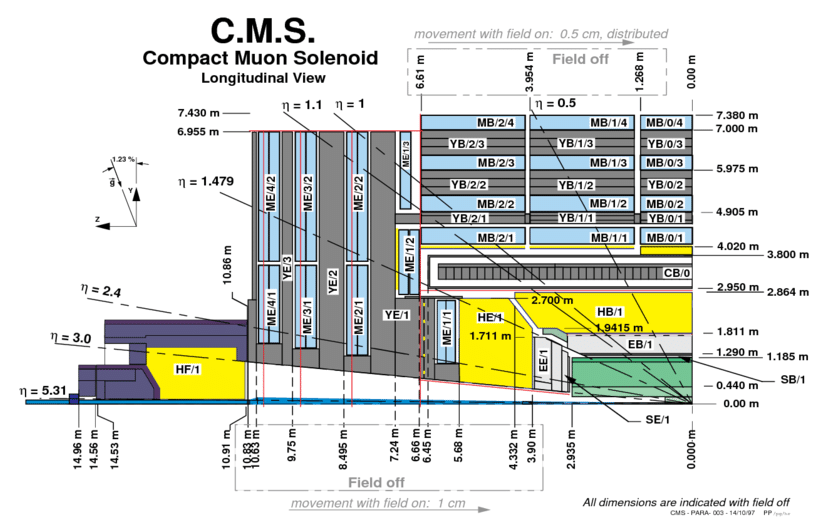
\includegraphics[width=\graphw, height=\graphh, keepaspectratio]{\PhDthesisdir/tex/slides/LHC-CMS/CMS/CMS-eta-ranges.png}
\end{center}
\end{frame}

\begin{frame}
\frametitle{Avoiding misidentification: Particles isolation -- qualitatively}
\begin{center}
\begin{tikzpicture}
\def\trackerrin{.100}
\def\trackerrout{1.185}
\def\trackercolor{ltcolorgray1}

\def\ECALrin{1.290}
\def\ECALrout{1.811}
\def\ECALcolor{ltcolorgreen1}

\def\HCALrin{1.812}
\def\HCALrout{2.854}
\def\HCALcolor{ltcoloryellow3}

\def\Solenrin{2.950}
\def\Solenrout{3.800}
\def\Solencolor{ltcolorgray2}

\def\ironryrina{3.850}
\def\ironryrouta{4.000}
\def\muonrina{4.020}
\def\muonrouta{4.400}
\def\ironryrinb{4.420}
\def\ironryroutb{4.880}
\def\muonrinb{4.905}
\def\muonroutb{5.285}
\def\ironryrinc{5.300}
\def\ironryroutc{5.960}
\def\muonrinc{5.975}
\def\muonroutc{6.355}
\def\ironryrind{6.375}
\def\ironryroutd{6.980}
\def\muonrind{7.000}
\def\muonroutd{7.380}
\def\muoncolor{ltcoloryellow1}
\def\ironrycolor{ltcolorred3}

\clip (-\graphw/2,-\graphh/2) rectangle (\graphw/2,\graphh/2);

\draw (0,0) coordinate (PV);

\foreach \rin/\rout/\color in {
\muonrind/\muonroutd/\muoncolor,
\ironryrind/\ironryroutd/\ironrycolor,
\muonrinc/\muonroutc/\muoncolor,
\ironryrinc/\ironryroutc/\ironrycolor,
\muonrinb/\muonroutb/\muoncolor,
\ironryrinb/\ironryroutb/\ironrycolor,
\muonrina/\muonrouta/\muoncolor,
%\ironryrina/\ironryrouta/\ironrycolor,
\Solenrin/\Solenrout/\Solencolor,
\HCALrin/\HCALrout/\HCALcolor,
\ECALrin/\ECALrout/\ECALcolor,
\trackerrin/\trackerrout/\trackercolor
}{
\fill (PV) [color = \color] circle (\rout);
\fill (PV) [color = white] circle (\rin);
}

\foreach \phiangle/\maxradius/\linecolor/\linethick in {
150/\HCALrin/ltcolorgreen/thin,
120/\HCALrin/ltcolorred/very thick,
122/\HCALrin/ltcolorred/thin,
117/\HCALrin/ltcolorred/thin,
0/\HCALrin/ltcolorblue/very thick,
5/\ECALrin/ltcolorblue/thin,
10/\HCALrin/ltcolorblue/thin,
-7/\ECALrin/ltcolorblue/thin,
-13/\HCALrin/ltcolorblue/thin,
8/\ECALrin/ltcolorblue/thin,
-2/\HCALrin/ltcolorblue/thin,
3/\ECALrin/ltcolorblue/thin}{
\draw [\linecolor, \linethick] (PV) --+ (\phiangle:\trackerrout);
\def\newmaxradius{\maxradius+.25}
\ifthenelse{\equal{\maxradius}{\ECALrin}}{\def\newmaxradius{\ECALrout}}{}
\ifthenelse{\equal{\maxradius}{\HCALrin}}{\def\newmaxradius{\HCALrout}}{}
\draw [\linecolor4, ultra thick] (PV)+(\phiangle:\maxradius)--+(\phiangle:\newmaxradius);
}

\end{tikzpicture}
\end{center}
\end{frame}

\begin{frame}\addtocounter{framenumber}{-1}
\frametitle{Avoiding misidentification: Particles isolation -- quantitatively}
\begin{block}{}
\begin{equation*}
I_\text{rel}^{(\ell)}
=
\left.
\frac{1}{p_T^{(\ell)}}
\left[
\sum_{\hadron^\pm,\text{PV}} p_T^{\hadron^\pm}
+
\max\left(
0
,
\sum_{\hadron^0}p_{\hadron^0}
+
\sum_{\gamma}p_{\gamma}
- \Delta\beta
\sum_{\hadron^\pm,\text{PU}} p_T^{\hadron^\pm}
\right)
\right]
\right|_{\Delta R < R_\ell}
\end{equation*}
\begin{center}
with $\Delta R = \sqrt{\Delta\phi^2+\Delta\eta^2}$.
\end{center}
\end{block}
\pause
\begin{block}{Particles isolation cut for SR}
\begin{itemize}
\item[$\ell$] $I_\text{rel}<\num{0.3}$,
$R_\ell = \num{0.5}$.
\item[\tauh] MVA-based isolation criterion with 3 available WP:
\begin{itemize}
\item Very Loose (VLoose),
\item Medium,
\item Tight (used for SR).
\end{itemize}
\end{itemize}
\end{block}
\end{frame}

\begin{frame}
\frametitle{Signal region (SR) for semi-leptonic channels ($\ell\tauh$)}

\begin{block}{Obtaining \emph{dileptons} candidates}
\begin{minipage}[c]{.55\linewidth}
With all $L_1$ and $L_2$ passing selection,\\
compose  pairs ($L_1L_2$) respecting:
\begin{itemize}
\item opposed electric charges:\\ the initial Higgs is \textbf{neutral}.
\item pair separation $\Delta R > \num{0.5}$:\\ avoid fake dileptons from jet particles.
\end{itemize}
\end{minipage}
\begin{minipage}[c]{.4\linewidth}
\begin{fmffile}{H-tautau_small}\fmfstraight
\begin{fmfchar*}(40,30)
  \fmfleft{h}
  \fmfright{tau1,tau2}
  \fmf{dashes, label=$\Hs,, \Hn,, \Ha$, l.side=left}{h,v}
  \fmf{fermion, label=$\tau^+$, l.side=left}{tau1,v}
  \fmf{fermion, label=$\tau^-$, l.side=left}{v,tau2}
  \fmfdot{v}
\end{fmfchar*}
\end{fmffile}
\end{minipage}
\end{block}
\pause
\begin{block}{Selecting one dilepton}
Choose by:\\
~\hfill
most isolated $L_1$,
\hfill
highest $\pT^{L_1}$,
\hfill
most isolated $L_2$,
\hfill
highest $\pT^{L_2}$.
\hfill~
\end{block}

\end{frame}


\begin{frame}
\frametitle{Signal region (SR) for semi-leptonic channels ($\ell\tauh$)}

\begin{block}{Extra leptons}
\begin{center}
\begin{tabular}{ccccc}
\toprule
Variable & Dilepton (\mu) & 3\up{rd} lepton (\mu) & Dilepton (\ele) & 3\up{rd} lepton (\ele) \\
\midrule
$p_T^{(\ell')}$ & $>\SI{15}{GeV}$ & $>\SI{10}{GeV}$ & $>\SI{15}{GeV}$ & $>\SI{10}{GeV}$\\
$\eta^{(\ell')}$ & $<\num{2.4}$ & $<\num{2.4}$ & $<\num{2.5}$ & $<\num{2.5}$\\
\bottomrule
\end{tabular}
%\quad
%\begin{tabular}{ccc}
%\toprule
%Grandeur & Dilepton (\ele) & 3\up{e} lepton (\ele) \\
%\midrule
%$p_T^{(\ele')}$ & $>\SI{15}{GeV}$ & $>\SI{10}{GeV}$ \\
%$\eta^{(\ele')}$ & $<\num{2.5}$ & $<\num{2.5}$\\
%\bottomrule
%\end{tabular}
\end{center}
\end{block}

\pause
\begin{block}{Transverse mass}
\begin{equation*}
m_T^{(\ell)}<\SI{50}{GeV}
\msep
m_T^{(\ell)} = \sqrt{2p_T^{(\ell)} E_T^\text{miss}(1-\cos\Delta\phi)}
\end{equation*}
\end{block}
\end{frame}


\subsection*{Datasets}
%\begin{frame}
\frametitle{Datasets}

\begin{block}{Observed data (MiniAOD)}
\begin{minipage}[t]{.49\linewidth}
\begin{itemize}
\item \tauh\tauh
\begin{itemize}
\item \texttt{/Tau/Run2016[B-H]}
\item \texttt{/Tau/Run2017[B-F]}
\item \texttt{/Tau/Run2018[A-D]}
\end{itemize}
\item \ele\mu
\begin{itemize}
\item \texttt{/MuonEG/Run2016[B-H]}
\item \texttt{/MuonEG/Run2017[B-F]}
\item \texttt{/MuonEG/Run2018[A-D]}
\end{itemize}
\end{itemize}
\end{minipage}
\begin{minipage}[t]{.49\linewidth}
\begin{itemize}
\item \mu\tauh
\begin{itemize}
\item \texttt{/SingleMuon/Run2016[B-H]}
\item \texttt{/SingleMuon/Run2017[B-F]}
\item \texttt{/SingleMuon/Run2018[A-D]}
\end{itemize}
\item \ele\tauh
\begin{itemize}
\item \texttt{/SingleElectron/Run2016[B-H]}
\item \texttt{/SingleElectron/Run2017[B-F]}
\item \texttt{/EGamma/Run2018[A-D]}
\end{itemize}
\end{itemize}
\end{minipage}
\end{block}

\begin{center}
\footnotesize
\up{*}.\quad
More precisions on the exact datasets (date, version) in the manuscript!
\end{center}
\end{frame}

\begin{frame}
\frametitle{Datasets}

\begin{block}{Simulated signals (MiniAODSIM)}
\begin{itemize}
\item SM Higgs signals
\begin{itemize}
\item \texttt{/GluGlu\textbf{\color{ltcolorred}HToTauTau}\_M125\_13TeV\_powheg\_pythia8}
\item \texttt{/VBF\textbf{\color{ltcolorred}HToTauTau}\_M125\_13TeV\_powheg\_pythia8}
\item \texttt{/Wplus\textbf{\color{ltcolorred}HToTauTau}\_M125\_13TeV\_powheg\_pythia8}
\item \texttt{/Wminus\textbf{\color{ltcolorred}HToTauTau}\_M125\_13TeV\_powheg\_pythia8}
\item \texttt{/ggZH\_\textbf{\color{ltcolorred}HToTauTau}\_ZToLL\_M125\_13TeV\_powheg\_pythia8}
\item \texttt{/ggZH\_\textbf{\color{ltcolorred}HToTauTau}\_ZToNuNu\_M125\_13TeV\_powheg\_pythia8}
\item \texttt{/ggZH\_\textbf{\color{ltcolorred}HToTauTau}\_ZToQQ\_M125\_13TeV\_powheg\_pythia8}
\end{itemize}
\item MSSM signals
\begin{itemize}
\item \texttt{/\textbf{\color{ltcolorred}SUSY}GluGluTo\textbf{\color{ltcolorred}HToTauTau}\_M-*\_TuneCUETP8M1\_13TeV-pythia8}
\item \texttt{/\textbf{\color{ltcolorred}SUSY}GluGluTo\textbf{\color{ltcolorred}BBHToTauTau}\_M-*\_TuneCUETP8M1\_13TeV-amcatnlo-pythia8}
\end{itemize}
\end{itemize}
\end{block}
\end{frame}


\begin{frame}
\begin{center}
\LARGE Background processes?
\end{center}
\end{frame}

\begin{frame}
\frametitle{Backgrounds: Drell-Yan}

\begin{minipage}[c]{.45\textwidth}
\begin{block}{Drell-Yan (especially $\Zboson\to\tau\tau$)\vphantom{ÀQj}}
\begin{center}
\begin{tikzpicture}
\def\trackerrin{.100}
\def\trackerrout{1.185}
\def\trackercolor{ltcolorgray1}

\def\ECALrin{1.290}
\def\ECALrout{1.811}
\def\ECALcolor{ltcolorgreen1}

\def\HCALrin{1.812}
\def\HCALrout{2.854}
\def\HCALcolor{ltcoloryellow3}

\def\Solenrin{2.950}
\def\Solenrout{3.800}
\def\Solencolor{ltcolorgray2}

\def\ironryrina{3.850}
\def\ironryrouta{4.000}
\def\muonrina{4.020}
\def\muonrouta{4.400}
\def\ironryrinb{4.420}
\def\ironryroutb{4.880}
\def\muonrinb{4.905}
\def\muonroutb{5.285}
\def\ironryrinc{5.300}
\def\ironryroutc{5.960}
\def\muonrinc{5.975}
\def\muonroutc{6.355}
\def\ironryrind{6.375}
\def\ironryroutd{6.980}
\def\muonrind{7.000}
\def\muonroutd{7.380}
\def\muoncolor{ltcoloryellow1}
\def\ironrycolor{ltcolorred2}

\def\printele#1{
\draw [thick, ltcolorred] (0,0) arc (#1-90:#1-90+27:3) coordinate (eledeposit);
\draw [ltcolorred] (#1-5:1.25) node {\ele};
}
\def\printmu#1{
\draw [thick, ltcolorblue] (0,0) arc (#1-90:#1-90+33:6) arc (#1-90+33:#1-90:-12) node{\mu};
\draw [ltcolorblue] (#1-7:1.5) node {\mu};
}

\def\printantiele#1{
\draw [thick, ltcolorred] (0,0) arc (#1-90:#1-90-27:-3) coordinate (eledeposit);
\draw [ltcolorred] (#1-7:1.5) node {\ele};
%\draw [ltcolorred4, ultra thick] (eledeposit)--+(#1+25:\ECALrout);
}
\def\printantimu#1{
\draw [thick, ltcolorblue] (0,0) arc (#1-90:#1-90-33:-6) arc (#1-90-33:#1-90:12);
\draw [ltcolorblue] (#1-7:1.5) node {\mu};
}

\def\printtauh#1{
\draw [thick, ltcolorgreen4] (0,0) arc (#1-90:#1-90+11:10) ;
\draw [thick, ltcolorgreen4] (0,0) arc (#1-90:#1-90+6:20) ;
\draw [thick, ltcolorgreen4] (0,0) arc (#1-90:#1-90-11:-10) ;
\draw [ltcolorgreen4] (#1-12:1.5) node {\tauh};
}
\def\printantitauh#1{
\draw [thick, ltcolorgreen4] (0,0) arc (#1-90:#1-90-11:-10) ;
\draw [thick, ltcolorgreen4] (0,0) arc (#1-90:#1-90-6:-20) ;
\draw [thick, ltcolorgreen4] (0,0) arc (#1-90:#1-90+11:10) ;
\draw [ltcolorgreen4] (#1-12:1.5) node {\tauh};
}

\def\printjetnolabel#1{
\draw [thick, ltcolororange] (0,0) arc (#1-90+10:#1-90+22+10:5) ;
\draw [thick, ltcolororange] (0,0) arc (#1-90+5:#1-90+12+5:10) ;
\draw [thick, ltcolororange] (0,0) arc (#1-90:#1-90-22:-5) ;
\draw [thick, ltcolororange] (0,0) arc (#1-90:#1-90+6:20) ;
\draw [thick, ltcolororange] (0,0) arc (#1-90+5:#1-90+8+5:10) ;
\draw [thick, ltcolororange] (0,0) arc (#1-90:#1-90-11:-10) ;
\draw [thick, ltcolororange] (0,0) arc (#1-90:#1-90+11:10) ;
}

\def\printjet#1{
\printjetnolabel{#1}
\draw [ltcolororange] (#1-25:.5) node {jet};
}

\def\printjetfake#1{
\printjet{#1}
\draw [thick, ltcolorgreen4] (0,0) arc (#1-90:#1-90+11:10) ;
\draw [thick, ltcolorgreen4] (0,0) arc (#1-90:#1-90+6:20) ;
\draw [thick, ltcolorgreen4] (0,0) arc (#1-90:#1-90-11:-10) ;
\draw [ltcolorgreen4] (#1-17:1.5) node {f.\tauh};
}

\def\printdeposit#1#2#3#4{
\fill [#1] (#2-2:#3) arc (#2-2:#2+2:#3) -- (#2+2:#4) arc (#2+2:#2-2:#4) ;
}

\def\printECALdeposit#1#2{\printdeposit{#1}{#2}{\ECALrin}{\ECALrout}}
\def\printHCALdeposit#1#2{\printdeposit{#1}{#2}{\HCALrin}{\HCALrout}}

\def\printtauhdeposit#1{
\printHCALdeposit{ltcoloryellow4}{#1+3}
\printHCALdeposit{ltcoloryellow4}{#1+5}
\printHCALdeposit{ltcoloryellow4}{#1-5}
}

\def\printjetdeposit#1{
\printHCALdeposit{ltcoloryellow4}{#1+3}
\printHCALdeposit{ltcoloryellow4}{#1+5}
\printHCALdeposit{ltcoloryellow4}{#1-5}
\printHCALdeposit{ltcoloryellow4}{#1+21}
\printHCALdeposit{ltcoloryellow4}{#1+11}
\printHCALdeposit{ltcoloryellow4}{#1-11}
}

\def\printMuChSigA#1#2{
\fill [red] (#1-7.5+20*#2:\muonrina) arc (#1-7.5+20*#2:#1+7.5+20*#2:\muonrina) -- (#1+7.5+20*#2:\muonrouta) arc (#1+7.5+20*#2:#1-7.5+20*#2:\muonrouta) ;
}
\def\printMuChSigB#1#2{
\fill [red] (#1-7.5+20*#2:\muonrinb) arc (#1-7.5+20*#2:#1+7.5+20*#2:\muonrinb) -- (#1+7.5+20*#2:\muonroutb) arc (#1+7.5+20*#2:#1-7.5+20*#2:\muonroutb) ;
}
\def\printMuChSigC#1#2{
\fill [red] (#1-7.5+20*#2:\muonrinc) arc (#1-7.5+20*#2:#1+7.5+20*#2:\muonrinc) -- (#1+7.5+20*#2:\muonroutc) arc (#1+7.5+20*#2:#1-7.5+20*#2:\muonroutc) ;
}
\def\printMuChSigD#1#2{
\fill [red] (#1-7.5+20*#2:\muonrind) arc (#1-7.5+20*#2:#1+7.5+20*#2:\muonrind) -- (#1+7.5+20*#2:\muonroutd) arc (#1+7.5+20*#2:#1-7.5+20*#2:\muonroutd) ;
}
\clip (-.4\textwidth,-.4\textwidth) rectangle (.4\textwidth,.4\textwidth);
\fill (0,0) circle (2pt);
\printmu{-10}
\printantitauh{150}
\end{tikzpicture}
\end{center}
\end{block}
\end{minipage}
\hfill
\begin{minipage}[c]{.45\textwidth}
\begin{block}{$\Higgs\to\tau\tau\to\mu\tauh$\vphantom{ÀQj}}
\begin{center}
\begin{tikzpicture}
\def\trackerrin{.100}
\def\trackerrout{1.185}
\def\trackercolor{ltcolorgray1}

\def\ECALrin{1.290}
\def\ECALrout{1.811}
\def\ECALcolor{ltcolorgreen1}

\def\HCALrin{1.812}
\def\HCALrout{2.854}
\def\HCALcolor{ltcoloryellow3}

\def\Solenrin{2.950}
\def\Solenrout{3.800}
\def\Solencolor{ltcolorgray2}

\def\ironryrina{3.850}
\def\ironryrouta{4.000}
\def\muonrina{4.020}
\def\muonrouta{4.400}
\def\ironryrinb{4.420}
\def\ironryroutb{4.880}
\def\muonrinb{4.905}
\def\muonroutb{5.285}
\def\ironryrinc{5.300}
\def\ironryroutc{5.960}
\def\muonrinc{5.975}
\def\muonroutc{6.355}
\def\ironryrind{6.375}
\def\ironryroutd{6.980}
\def\muonrind{7.000}
\def\muonroutd{7.380}
\def\muoncolor{ltcoloryellow1}
\def\ironrycolor{ltcolorred2}

\def\printele#1{
\draw [thick, ltcolorred] (0,0) arc (#1-90:#1-90+27:3) coordinate (eledeposit);
\draw [ltcolorred] (#1-5:1.25) node {\ele};
}
\def\printmu#1{
\draw [thick, ltcolorblue] (0,0) arc (#1-90:#1-90+33:6) arc (#1-90+33:#1-90:-12) node{\mu};
\draw [ltcolorblue] (#1-7:1.5) node {\mu};
}

\def\printantiele#1{
\draw [thick, ltcolorred] (0,0) arc (#1-90:#1-90-27:-3) coordinate (eledeposit);
\draw [ltcolorred] (#1-7:1.5) node {\ele};
%\draw [ltcolorred4, ultra thick] (eledeposit)--+(#1+25:\ECALrout);
}
\def\printantimu#1{
\draw [thick, ltcolorblue] (0,0) arc (#1-90:#1-90-33:-6) arc (#1-90-33:#1-90:12);
\draw [ltcolorblue] (#1-7:1.5) node {\mu};
}

\def\printtauh#1{
\draw [thick, ltcolorgreen4] (0,0) arc (#1-90:#1-90+11:10) ;
\draw [thick, ltcolorgreen4] (0,0) arc (#1-90:#1-90+6:20) ;
\draw [thick, ltcolorgreen4] (0,0) arc (#1-90:#1-90-11:-10) ;
\draw [ltcolorgreen4] (#1-12:1.5) node {\tauh};
}
\def\printantitauh#1{
\draw [thick, ltcolorgreen4] (0,0) arc (#1-90:#1-90-11:-10) ;
\draw [thick, ltcolorgreen4] (0,0) arc (#1-90:#1-90-6:-20) ;
\draw [thick, ltcolorgreen4] (0,0) arc (#1-90:#1-90+11:10) ;
\draw [ltcolorgreen4] (#1-12:1.5) node {\tauh};
}

\def\printjetnolabel#1{
\draw [thick, ltcolororange] (0,0) arc (#1-90+10:#1-90+22+10:5) ;
\draw [thick, ltcolororange] (0,0) arc (#1-90+5:#1-90+12+5:10) ;
\draw [thick, ltcolororange] (0,0) arc (#1-90:#1-90-22:-5) ;
\draw [thick, ltcolororange] (0,0) arc (#1-90:#1-90+6:20) ;
\draw [thick, ltcolororange] (0,0) arc (#1-90+5:#1-90+8+5:10) ;
\draw [thick, ltcolororange] (0,0) arc (#1-90:#1-90-11:-10) ;
\draw [thick, ltcolororange] (0,0) arc (#1-90:#1-90+11:10) ;
}

\def\printjet#1{
\printjetnolabel{#1}
\draw [ltcolororange] (#1-25:.5) node {jet};
}

\def\printjetfake#1{
\printjet{#1}
\draw [thick, ltcolorgreen4] (0,0) arc (#1-90:#1-90+11:10) ;
\draw [thick, ltcolorgreen4] (0,0) arc (#1-90:#1-90+6:20) ;
\draw [thick, ltcolorgreen4] (0,0) arc (#1-90:#1-90-11:-10) ;
\draw [ltcolorgreen4] (#1-17:1.5) node {f.\tauh};
}

\def\printdeposit#1#2#3#4{
\fill [#1] (#2-2:#3) arc (#2-2:#2+2:#3) -- (#2+2:#4) arc (#2+2:#2-2:#4) ;
}

\def\printECALdeposit#1#2{\printdeposit{#1}{#2}{\ECALrin}{\ECALrout}}
\def\printHCALdeposit#1#2{\printdeposit{#1}{#2}{\HCALrin}{\HCALrout}}

\def\printtauhdeposit#1{
\printHCALdeposit{ltcoloryellow4}{#1+3}
\printHCALdeposit{ltcoloryellow4}{#1+5}
\printHCALdeposit{ltcoloryellow4}{#1-5}
}

\def\printjetdeposit#1{
\printHCALdeposit{ltcoloryellow4}{#1+3}
\printHCALdeposit{ltcoloryellow4}{#1+5}
\printHCALdeposit{ltcoloryellow4}{#1-5}
\printHCALdeposit{ltcoloryellow4}{#1+21}
\printHCALdeposit{ltcoloryellow4}{#1+11}
\printHCALdeposit{ltcoloryellow4}{#1-11}
}

\def\printMuChSigA#1#2{
\fill [red] (#1-7.5+20*#2:\muonrina) arc (#1-7.5+20*#2:#1+7.5+20*#2:\muonrina) -- (#1+7.5+20*#2:\muonrouta) arc (#1+7.5+20*#2:#1-7.5+20*#2:\muonrouta) ;
}
\def\printMuChSigB#1#2{
\fill [red] (#1-7.5+20*#2:\muonrinb) arc (#1-7.5+20*#2:#1+7.5+20*#2:\muonrinb) -- (#1+7.5+20*#2:\muonroutb) arc (#1+7.5+20*#2:#1-7.5+20*#2:\muonroutb) ;
}
\def\printMuChSigC#1#2{
\fill [red] (#1-7.5+20*#2:\muonrinc) arc (#1-7.5+20*#2:#1+7.5+20*#2:\muonrinc) -- (#1+7.5+20*#2:\muonroutc) arc (#1+7.5+20*#2:#1-7.5+20*#2:\muonroutc) ;
}
\def\printMuChSigD#1#2{
\fill [red] (#1-7.5+20*#2:\muonrind) arc (#1-7.5+20*#2:#1+7.5+20*#2:\muonrind) -- (#1+7.5+20*#2:\muonroutd) arc (#1+7.5+20*#2:#1-7.5+20*#2:\muonroutd) ;
}
\clip (-.4\textwidth,-.4\textwidth) rectangle (.4\textwidth,.4\textwidth);
\fill (0,0) circle (2pt);
\printmu{-10}
\printantitauh{150}
\end{tikzpicture}
\end{center}
\end{block}
\end{minipage}

%\begin{block}{Drell-Yan}
%\hfill
%\begin{minipage}[c]{.45\textwidth}
%\vspace{\baselineskip}
%
%\begin{fmffile}{DY}\fmfstraight
\begin{fmfchar*}(50,25)
  \fmfleft{pi1,pi2}
  \fmfright{po1,l1,l2,po2}
  \fmf{fermion, label=$p$, l.side=left, tension=3}{pi1,v1}
  \fmf{fermion, label=$p$, l.side=right, tension=3}{pi2,v2}
  \fmf{phantom}{v1,po1}
  \fmf{phantom}{v2,po2}
  \fmffreeze
  \fmf{fermion}{v1,v3,v2}
  \fmf{boson, label=$Z/\gamma^*$, l.side=left, tension =3}{v3,v4}
  \fmf{fermion}{l1,v4,l2}
  \fmfdot{v3,v4}
  \fmfblob{.1w}{v1,v2}
  \fmflabel{$\bar{f}$}{l1}
  \fmflabel{$f$}{l2}
  \fmffreeze
  \fmfi{plain}{vpath (__pi1,__v1) shifted (thick*(0,2))}
  \fmfi{plain}{vpath (__pi1,__v1) shifted (thick*(0,-2))}
  \fmfi{plain}{vpath (__pi2,__v2) shifted (thick*(0,2))}
  \fmfi{plain}{vpath (__pi2,__v2) shifted (thick*(0,-2))}
  \fmfi{fermion}{vpath (__v1,__po1) shifted (thick*(0,1.5))}
  \fmfi{fermion}{vpath (__v1,__po1) shifted (thick*(0,-1.5))}
  \fmfi{fermion}{vpath (__v2,__po2) shifted (thick*(0,1.5))}
  \fmfi{fermion}{vpath (__v2,__po2) shifted (thick*(0,-1.5))}
\end{fmfchar*}
\end{fmffile}
%
%~
%\end{minipage}
%\hfill
%\begin{minipage}[c]{.4\linewidth}
%\begin{itemize}
%\item $f\bar{f} = \leptau\antitau$ fakes $\Higgs\to\tau\tau$
%\item $Z\to\ell\ell$ and a $\ell$ fakes a \tauh
%\end{itemize}
%\end{minipage}
%\end{block}

\end{frame}
\addtocounter{framenumber}{-1}
\def\EmbedPictsWidth{2.5}
\def\EmbedPictsMargin{.8}
\def\EmbedPictsTxtSize{}
\begin{frame}
\backupslinklabel{emb}
\frametitle{Embedded events \& genuine \tau\ leptons}\beamercite{embedding}
\begin{center}\vspace{-.5\baselineskip}
\begin{tikzpicture}
\only<1->{
\draw (\EmbedPictsWidth/2, \EmbedPictsWidth) node [above] {\EmbedPictsTxtSize $\Zboson\to\mu\mu$ data};
\node[anchor=south west,inner sep=0] at (0,0) {\frame{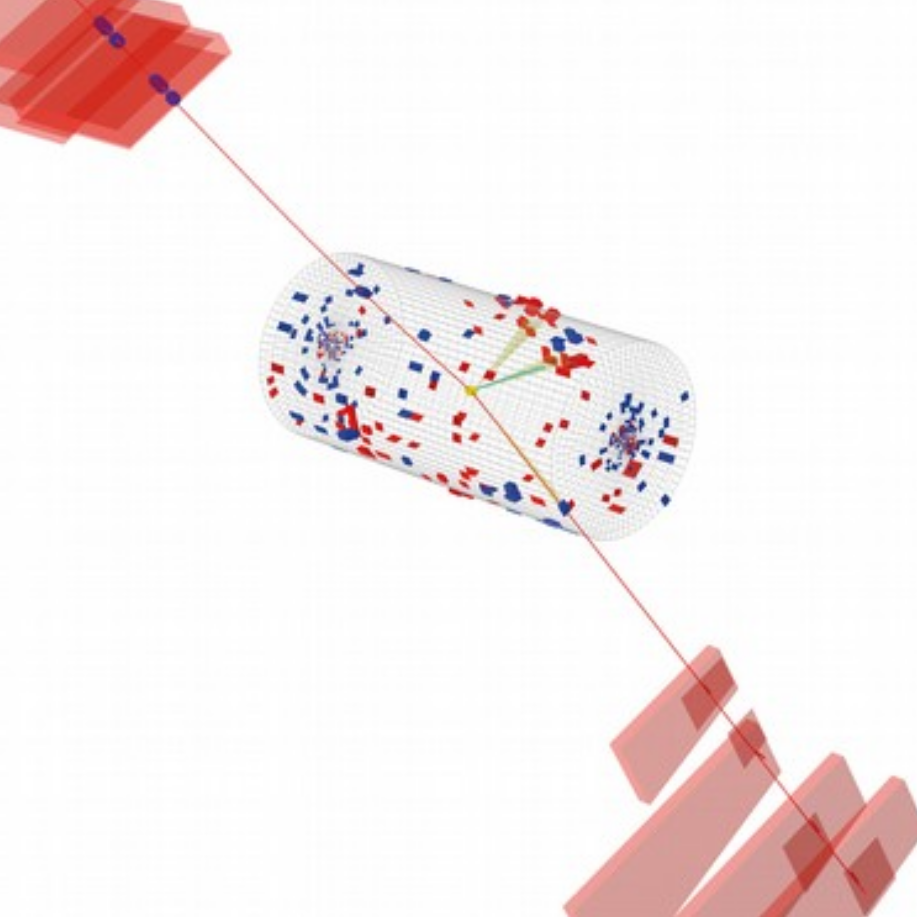
\includegraphics[width=\EmbedPictsWidth cm]{\PhDthesisdir/plots_and_images/from_embedding/Z_to_mumu_data.png}}};
}

\only<2->{
\draw [-latex, very thick] (\EmbedPictsWidth+\EmbedPictsMargin/5, \EmbedPictsWidth/2) -- + (3*\EmbedPictsMargin/5,0);
\draw (\EmbedPictsWidth/2+\EmbedPictsWidth+\EmbedPictsMargin, \EmbedPictsWidth) node [above] {\EmbedPictsTxtSize Remove $\mu\mu$ system};
\node[anchor=south west,inner sep=0] at (\EmbedPictsWidth+\EmbedPictsMargin,0) {\frame{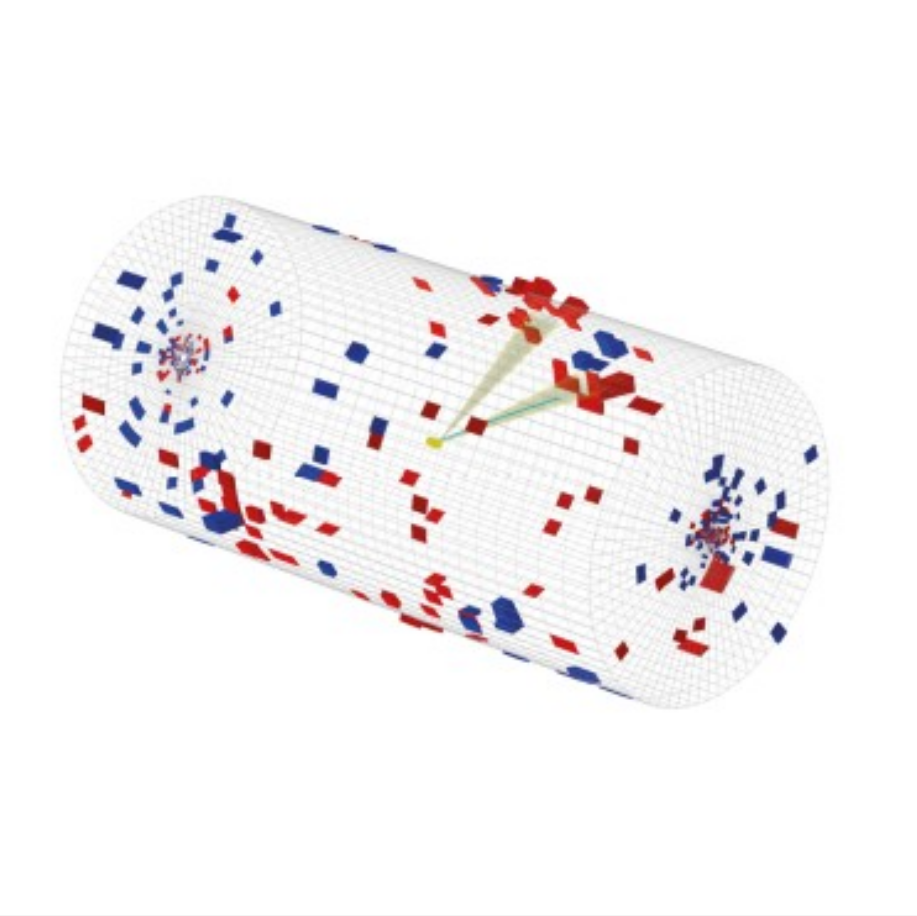
\includegraphics[width=\EmbedPictsWidth cm]{\PhDthesisdir/plots_and_images/from_embedding/remove_mumu.png}}};
}

\only<3->{
\draw (\EmbedPictsWidth+\EmbedPictsMargin,-\EmbedPictsWidth/2-\EmbedPictsMargin) node [above left] {\EmbedPictsTxtSize Simulate $\Zboson\to\tau\tau$};
\draw (\EmbedPictsWidth+\EmbedPictsMargin,-\EmbedPictsWidth/2-\EmbedPictsMargin) node [below left] {\EmbedPictsTxtSize ($\vec{p}_{\tau} \simeq \vec{p}_{\mu}$)};
\node[anchor=south west,inner sep=0] at (\EmbedPictsWidth+\EmbedPictsMargin,-\EmbedPictsWidth-\EmbedPictsMargin) {\frame{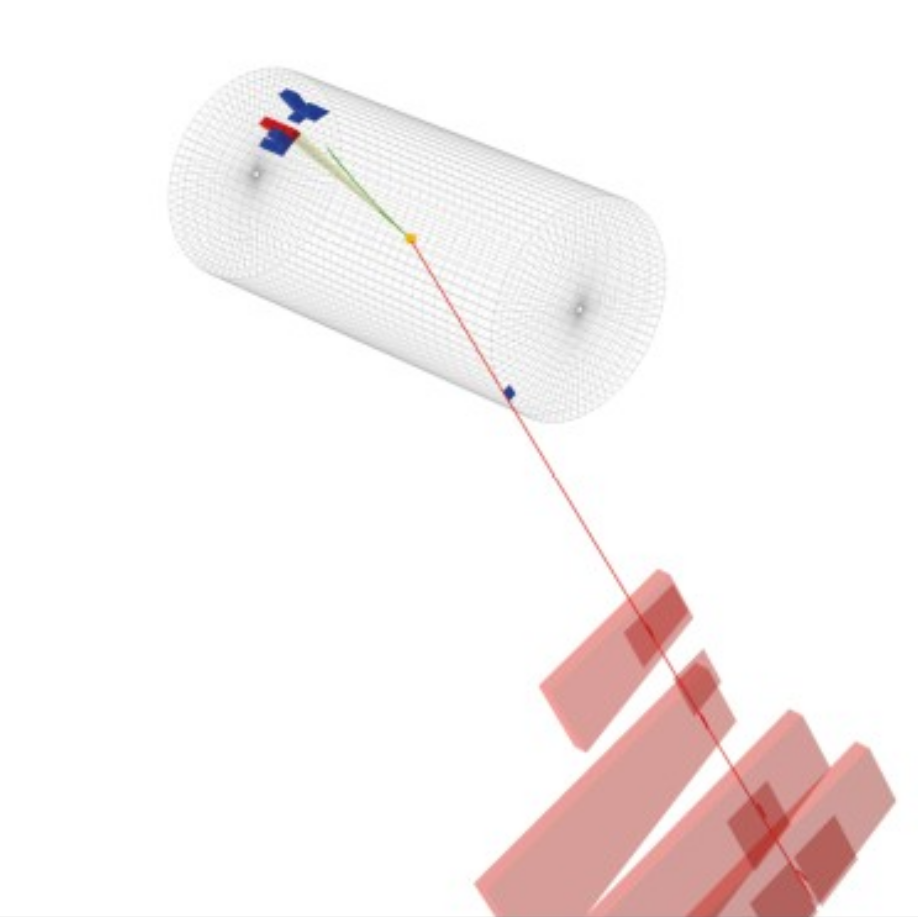
\includegraphics[width=\EmbedPictsWidth cm]{\PhDthesisdir/plots_and_images/from_embedding/Z_to_tautau_simulation.png}}};
}

\only<4->{
\draw [-latex, very thick] (2*\EmbedPictsWidth+6*\EmbedPictsMargin/5, \EmbedPictsWidth/4) -- (2*\EmbedPictsWidth+2*\EmbedPictsMargin-\EmbedPictsMargin/5,0);
\draw [-latex, very thick] (2*\EmbedPictsWidth+6*\EmbedPictsMargin/5,-\EmbedPictsWidth/4-\EmbedPictsMargin) -- (2*\EmbedPictsWidth+2*\EmbedPictsMargin-\EmbedPictsMargin/5,-\EmbedPictsMargin);
\draw (2*\EmbedPictsWidth+2*\EmbedPictsMargin+\EmbedPictsWidth/2,\EmbedPictsWidth/2-\EmbedPictsMargin/2) node [above] {\EmbedPictsTxtSize $\Zboson\to\tau\tau$ embedded event};
\node[anchor=south west,inner sep=0] at (2*\EmbedPictsWidth+2*\EmbedPictsMargin,-\EmbedPictsWidth/2-\EmbedPictsMargin/2) {\frame{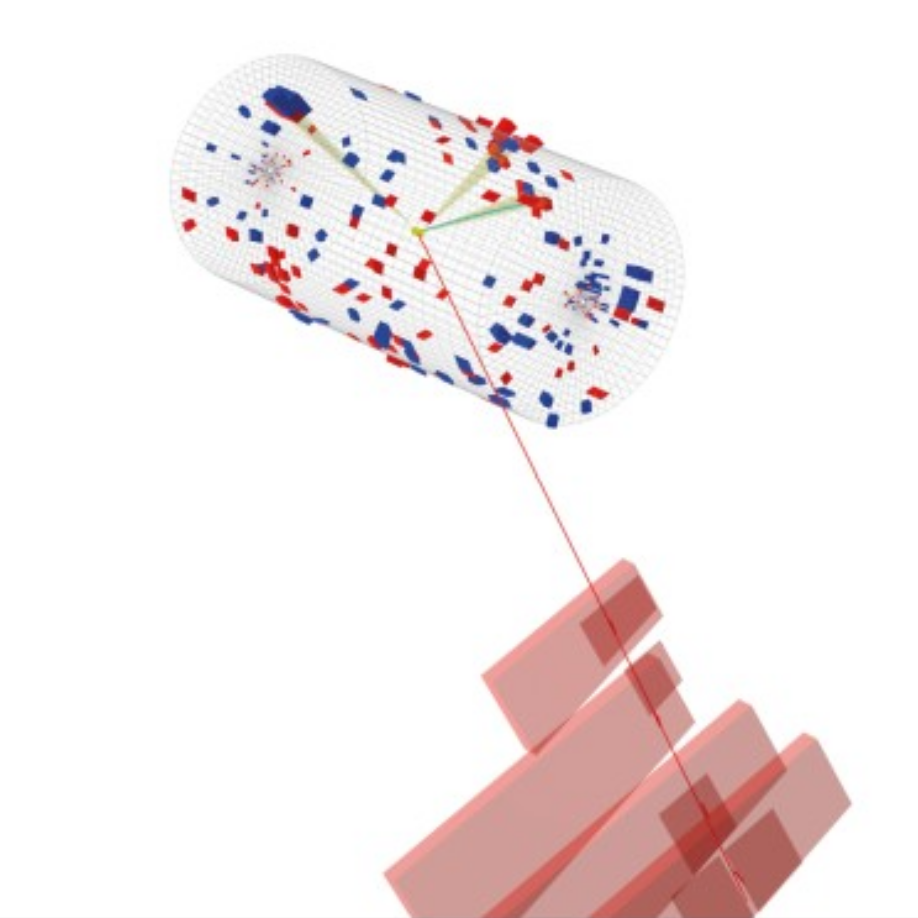
\includegraphics[width=\EmbedPictsWidth cm]{\PhDthesisdir/plots_and_images/from_embedding/embedded_event.png}}};
}

\clip (-1,-\EmbedPictsWidth-\EmbedPictsMargin-.25) rectangle (3*\EmbedPictsWidth+5*\EmbedPictsMargin/2+.25, \EmbedPictsWidth+.5);
\end{tikzpicture}
\end{center}\vspace{-.5\baselineskip}
\end{frame}
\begin{frame}
\frametitle{Backgrounds: $\Wboson+\text{jets}$}

%\begin{block}{$\Wboson+\text{jets}$}
%\Wboson\ fakes prompt letpon and a jet fakes a \tauh.
%\end{block}

\begin{minipage}[c]{.45\textwidth}
\begin{block}{$\Wboson+\text{jets}$\vphantom{ÀQj}}
\begin{center}
\begin{tikzpicture}
\clip (-.4\textwidth,-.2\textwidth) rectangle (.4\textwidth,.25\textwidth);
\fill (0,0) circle (2pt);
\printantimuon{7}{10}
\printjet{9}{150}
\end{tikzpicture}
\end{center}
\end{block}
\end{minipage}
\hfill
\begin{minipage}[c]{.45\textwidth}
\begin{block}{$\Higgs\to\tau\tau\to\mu\tauh$\vphantom{ÀQj}}
\begin{center}
\begin{tikzpicture}
\clip (-.4\textwidth,-.2\textwidth) rectangle (.4\textwidth,.25\textwidth);
\fill (0,0) circle (2pt);
\printantimuon{7}{10}
\printtauh{9}{150}
\end{tikzpicture}
\end{center}
\end{block}
\end{minipage}

%\begin{block}{}
%\begin{itemize}
%\item \texttt{/W[1-4]JetsToLNu\_TuneCP5\_13TeV-madgraphMLM-pythia8}
%\item \texttt{/WZTo2L2Q\_13TeV\_amcatnloFXFX\_madspin\_pythia8} ...
%\end{itemize}
%\end{block}

\end{frame}

\begin{frame}\addtocounter{framenumber}{-1}
\frametitle{Backgrounds: $\Wboson+\text{jets}$}

%\begin{block}{$\Wboson+\text{jets}$}
%\Wboson\ fakes prompt letpon and a jet fakes a \tauh.
%\end{block}

\begin{minipage}[c]{.45\textwidth}
\begin{block}{$\Wboson+\text{jets}$, $\text{jet}\to\text{fake \tauh}$\vphantom{ÀQj}}
\begin{center}
\begin{tikzpicture}
\clip (-.4\textwidth,-.2\textwidth) rectangle (.4\textwidth,.25\textwidth);
\fill (0,0) circle (2pt);
\printantimuon{7}{10}
\printjetfake{9}{150}
\end{tikzpicture}
\end{center}
\end{block}
\end{minipage}
\hfill
\begin{minipage}[c]{.45\textwidth}
\begin{block}{$\Higgs\to\tau\tau\to\mu\tauh$\vphantom{ÀQj}}
\begin{center}
\begin{tikzpicture}
\clip (-.4\textwidth,-.2\textwidth) rectangle (.4\textwidth,.25\textwidth);
\fill (0,0) circle (2pt);
\printantimuon{7}{10}
\printtauh{9}{150}
\end{tikzpicture}
\end{center}
\end{block}
\end{minipage}

%\begin{block}{}
%\begin{itemize}
%\item \texttt{/W[1-4]JetsToLNu\_TuneCP5\_13TeV-madgraphMLM-pythia8}
%\item \texttt{/WZTo2L2Q\_13TeV\_amcatnloFXFX\_madspin\_pythia8} ...
%\end{itemize}
%\end{block}

\end{frame}
\addtocounter{framenumber}{-1}
\begin{frame}
\frametitle{Backgrounds: \ttbar}
%\begin{block}{\ttbar}
%\quarkt\ decays by weak interation, faking weak decay of a \tau\ + \quarkb-jets.
%\end{block}

\begin{minipage}[c]{.45\textwidth}
\begin{block}{\ttbar\vphantom{ÀQj}}
\begin{center}
\begin{tikzpicture}
\clip (-.4\textwidth,-.3\textwidth) rectangle (.4\textwidth,.3\textwidth);
\fill (0,0) circle (2pt);
\printantimuon{7}{10}
\printtauh{9}{150}
\printjet{9}{-155}
\printjet{9}{45}
\end{tikzpicture}
\end{center}
\end{block}
\end{minipage}
\hfill
\begin{minipage}[c]{.45\textwidth}
\begin{block}{$\Higgs\to\tau\tau\to\mu\tauh$\vphantom{ÀQj}}
\begin{center}
\begin{tikzpicture}
\clip (-.4\textwidth,-.3\textwidth) rectangle (.4\textwidth,.3\textwidth);
\fill (0,0) circle (2pt);
\printantimuon{7}{10}
\printtauh{9}{150}
\end{tikzpicture}
\end{center}
\end{block}
\end{minipage}

\begin{block}{}
\begin{itemize}
\item \texttt{/TTToHadronic\_TuneCP5\_13TeV-powheg-pythia8}
\item \texttt{/TTToSemiLeptonic\_TuneCP5\_13TeV-powheg-pythia8} ...
\end{itemize}
\end{block}

\end{frame}

\begin{frame}\addtocounter{framenumber}{-1}
\frametitle{Backgrounds: \ttbar}

\begin{minipage}[c]{.45\textwidth}
\begin{block}{\ttbar\vphantom{ÀQj}}
\begin{center}
\begin{tikzpicture}
\clip (-.4\textwidth,-.3\textwidth) rectangle (.4\textwidth,.3\textwidth);
\fill (0,0) circle (2pt);
\printantimuon{7}{10}
\printtauh{9}{150}
\printjet{9}{-155}
\printjet{9}{45}
\end{tikzpicture}
\end{center}
\end{block}
\end{minipage}
\hfill
\begin{minipage}[c]{.45\textwidth}
\begin{block}{$\Higgs$ production with \quarkb-jets\vphantom{ÀQj}}
\begin{center}
\begin{tikzpicture}
\clip (-.4\textwidth,-.3\textwidth) rectangle (.4\textwidth,.3\textwidth);
\fill (0,0) circle (2pt);
\printantimuon{7}{10}
\printtauh{9}{150}
\printjet{9}{-155}
\printjet{9}{45}
\end{tikzpicture}
\end{center}
\end{block}
\end{minipage}

\begin{block}{}
\begin{itemize}
\item \texttt{/TTToHadronic\_TuneCP5\_13TeV-powheg-pythia8}
\item \texttt{/TTToSemiLeptonic\_TuneCP5\_13TeV-powheg-pythia8} ...
\end{itemize}
\end{block}

\end{frame}
\addtocounter{framenumber}{-1}
\begin{frame}
\frametitle{Backgrounds: QCD}

\begin{minipage}[c]{.45\textwidth}
\begin{block}{QCD}
\begin{center}
\begin{tikzpicture}
\def\trackerrin{.100}
\def\trackerrout{1.185}
\def\trackercolor{ltcolorgray1}

\def\ECALrin{1.290}
\def\ECALrout{1.811}
\def\ECALcolor{ltcolorgreen1}

\def\HCALrin{1.812}
\def\HCALrout{2.854}
\def\HCALcolor{ltcoloryellow3}

\def\Solenrin{2.950}
\def\Solenrout{3.800}
\def\Solencolor{ltcolorgray2}

\def\ironryrina{3.850}
\def\ironryrouta{4.000}
\def\muonrina{4.020}
\def\muonrouta{4.400}
\def\ironryrinb{4.420}
\def\ironryroutb{4.880}
\def\muonrinb{4.905}
\def\muonroutb{5.285}
\def\ironryrinc{5.300}
\def\ironryroutc{5.960}
\def\muonrinc{5.975}
\def\muonroutc{6.355}
\def\ironryrind{6.375}
\def\ironryroutd{6.980}
\def\muonrind{7.000}
\def\muonroutd{7.380}
\def\muoncolor{ltcoloryellow1}
\def\ironrycolor{ltcolorred2}

\def\printele#1{
\draw [thick, ltcolorred] (0,0) arc (#1-90:#1-90+27:3) coordinate (eledeposit);
\draw [ltcolorred] (#1-5:1.25) node {\ele};
}
\def\printmu#1{
\draw [thick, ltcolorblue] (0,0) arc (#1-90:#1-90+33:6) arc (#1-90+33:#1-90:-12) node{\mu};
\draw [ltcolorblue] (#1-7:1.5) node {\mu};
}

\def\printantiele#1{
\draw [thick, ltcolorred] (0,0) arc (#1-90:#1-90-27:-3) coordinate (eledeposit);
\draw [ltcolorred] (#1-7:1.5) node {\ele};
%\draw [ltcolorred4, ultra thick] (eledeposit)--+(#1+25:\ECALrout);
}
\def\printantimu#1{
\draw [thick, ltcolorblue] (0,0) arc (#1-90:#1-90-33:-6) arc (#1-90-33:#1-90:12);
\draw [ltcolorblue] (#1-7:1.5) node {\mu};
}

\def\printtauh#1{
\draw [thick, ltcolorgreen4] (0,0) arc (#1-90:#1-90+11:10) ;
\draw [thick, ltcolorgreen4] (0,0) arc (#1-90:#1-90+6:20) ;
\draw [thick, ltcolorgreen4] (0,0) arc (#1-90:#1-90-11:-10) ;
\draw [ltcolorgreen4] (#1-12:1.5) node {\tauh};
}
\def\printantitauh#1{
\draw [thick, ltcolorgreen4] (0,0) arc (#1-90:#1-90-11:-10) ;
\draw [thick, ltcolorgreen4] (0,0) arc (#1-90:#1-90-6:-20) ;
\draw [thick, ltcolorgreen4] (0,0) arc (#1-90:#1-90+11:10) ;
\draw [ltcolorgreen4] (#1-12:1.5) node {\tauh};
}

\def\printjetnolabel#1{
\draw [thick, ltcolororange] (0,0) arc (#1-90+10:#1-90+22+10:5) ;
\draw [thick, ltcolororange] (0,0) arc (#1-90+5:#1-90+12+5:10) ;
\draw [thick, ltcolororange] (0,0) arc (#1-90:#1-90-22:-5) ;
\draw [thick, ltcolororange] (0,0) arc (#1-90:#1-90+6:20) ;
\draw [thick, ltcolororange] (0,0) arc (#1-90+5:#1-90+8+5:10) ;
\draw [thick, ltcolororange] (0,0) arc (#1-90:#1-90-11:-10) ;
\draw [thick, ltcolororange] (0,0) arc (#1-90:#1-90+11:10) ;
}

\def\printjet#1{
\printjetnolabel{#1}
\draw [ltcolororange] (#1-25:.5) node {jet};
}

\def\printjetfake#1{
\printjet{#1}
\draw [thick, ltcolorgreen4] (0,0) arc (#1-90:#1-90+11:10) ;
\draw [thick, ltcolorgreen4] (0,0) arc (#1-90:#1-90+6:20) ;
\draw [thick, ltcolorgreen4] (0,0) arc (#1-90:#1-90-11:-10) ;
\draw [ltcolorgreen4] (#1-17:1.5) node {f.\tauh};
}

\def\printdeposit#1#2#3#4{
\fill [#1] (#2-2:#3) arc (#2-2:#2+2:#3) -- (#2+2:#4) arc (#2+2:#2-2:#4) ;
}

\def\printECALdeposit#1#2{\printdeposit{#1}{#2}{\ECALrin}{\ECALrout}}
\def\printHCALdeposit#1#2{\printdeposit{#1}{#2}{\HCALrin}{\HCALrout}}

\def\printtauhdeposit#1{
\printHCALdeposit{ltcoloryellow4}{#1+3}
\printHCALdeposit{ltcoloryellow4}{#1+5}
\printHCALdeposit{ltcoloryellow4}{#1-5}
}

\def\printjetdeposit#1{
\printHCALdeposit{ltcoloryellow4}{#1+3}
\printHCALdeposit{ltcoloryellow4}{#1+5}
\printHCALdeposit{ltcoloryellow4}{#1-5}
\printHCALdeposit{ltcoloryellow4}{#1+21}
\printHCALdeposit{ltcoloryellow4}{#1+11}
\printHCALdeposit{ltcoloryellow4}{#1-11}
}

\def\printMuChSigA#1#2{
\fill [red] (#1-7.5+20*#2:\muonrina) arc (#1-7.5+20*#2:#1+7.5+20*#2:\muonrina) -- (#1+7.5+20*#2:\muonrouta) arc (#1+7.5+20*#2:#1-7.5+20*#2:\muonrouta) ;
}
\def\printMuChSigB#1#2{
\fill [red] (#1-7.5+20*#2:\muonrinb) arc (#1-7.5+20*#2:#1+7.5+20*#2:\muonrinb) -- (#1+7.5+20*#2:\muonroutb) arc (#1+7.5+20*#2:#1-7.5+20*#2:\muonroutb) ;
}
\def\printMuChSigC#1#2{
\fill [red] (#1-7.5+20*#2:\muonrinc) arc (#1-7.5+20*#2:#1+7.5+20*#2:\muonrinc) -- (#1+7.5+20*#2:\muonroutc) arc (#1+7.5+20*#2:#1-7.5+20*#2:\muonroutc) ;
}
\def\printMuChSigD#1#2{
\fill [red] (#1-7.5+20*#2:\muonrind) arc (#1-7.5+20*#2:#1+7.5+20*#2:\muonrind) -- (#1+7.5+20*#2:\muonroutd) arc (#1+7.5+20*#2:#1-7.5+20*#2:\muonroutd) ;
}
\clip (-.4\textwidth,-.4\textwidth) rectangle (.4\textwidth,.4\textwidth);
\fill (0,0) circle (2pt);
\printjet{-10}
\printmu{-10}
%\printantitauh{150}
\printjet{150}
\end{tikzpicture}
\end{center}
\end{block}
\end{minipage}
\hfill
\begin{minipage}[c]{.45\textwidth}
\begin{block}{$\Higgs\to\tau\tau\to\mu\tauh$}
\begin{center}
\begin{tikzpicture}
\def\trackerrin{.100}
\def\trackerrout{1.185}
\def\trackercolor{ltcolorgray1}

\def\ECALrin{1.290}
\def\ECALrout{1.811}
\def\ECALcolor{ltcolorgreen1}

\def\HCALrin{1.812}
\def\HCALrout{2.854}
\def\HCALcolor{ltcoloryellow3}

\def\Solenrin{2.950}
\def\Solenrout{3.800}
\def\Solencolor{ltcolorgray2}

\def\ironryrina{3.850}
\def\ironryrouta{4.000}
\def\muonrina{4.020}
\def\muonrouta{4.400}
\def\ironryrinb{4.420}
\def\ironryroutb{4.880}
\def\muonrinb{4.905}
\def\muonroutb{5.285}
\def\ironryrinc{5.300}
\def\ironryroutc{5.960}
\def\muonrinc{5.975}
\def\muonroutc{6.355}
\def\ironryrind{6.375}
\def\ironryroutd{6.980}
\def\muonrind{7.000}
\def\muonroutd{7.380}
\def\muoncolor{ltcoloryellow1}
\def\ironrycolor{ltcolorred2}

\def\printele#1{
\draw [thick, ltcolorred] (0,0) arc (#1-90:#1-90+27:3) coordinate (eledeposit);
\draw [ltcolorred] (#1-5:1.25) node {\ele};
}
\def\printmu#1{
\draw [thick, ltcolorblue] (0,0) arc (#1-90:#1-90+33:6) arc (#1-90+33:#1-90:-12) node{\mu};
\draw [ltcolorblue] (#1-7:1.5) node {\mu};
}

\def\printantiele#1{
\draw [thick, ltcolorred] (0,0) arc (#1-90:#1-90-27:-3) coordinate (eledeposit);
\draw [ltcolorred] (#1-7:1.5) node {\ele};
%\draw [ltcolorred4, ultra thick] (eledeposit)--+(#1+25:\ECALrout);
}
\def\printantimu#1{
\draw [thick, ltcolorblue] (0,0) arc (#1-90:#1-90-33:-6) arc (#1-90-33:#1-90:12);
\draw [ltcolorblue] (#1-7:1.5) node {\mu};
}

\def\printtauh#1{
\draw [thick, ltcolorgreen4] (0,0) arc (#1-90:#1-90+11:10) ;
\draw [thick, ltcolorgreen4] (0,0) arc (#1-90:#1-90+6:20) ;
\draw [thick, ltcolorgreen4] (0,0) arc (#1-90:#1-90-11:-10) ;
\draw [ltcolorgreen4] (#1-12:1.5) node {\tauh};
}
\def\printantitauh#1{
\draw [thick, ltcolorgreen4] (0,0) arc (#1-90:#1-90-11:-10) ;
\draw [thick, ltcolorgreen4] (0,0) arc (#1-90:#1-90-6:-20) ;
\draw [thick, ltcolorgreen4] (0,0) arc (#1-90:#1-90+11:10) ;
\draw [ltcolorgreen4] (#1-12:1.5) node {\tauh};
}

\def\printjetnolabel#1{
\draw [thick, ltcolororange] (0,0) arc (#1-90+10:#1-90+22+10:5) ;
\draw [thick, ltcolororange] (0,0) arc (#1-90+5:#1-90+12+5:10) ;
\draw [thick, ltcolororange] (0,0) arc (#1-90:#1-90-22:-5) ;
\draw [thick, ltcolororange] (0,0) arc (#1-90:#1-90+6:20) ;
\draw [thick, ltcolororange] (0,0) arc (#1-90+5:#1-90+8+5:10) ;
\draw [thick, ltcolororange] (0,0) arc (#1-90:#1-90-11:-10) ;
\draw [thick, ltcolororange] (0,0) arc (#1-90:#1-90+11:10) ;
}

\def\printjet#1{
\printjetnolabel{#1}
\draw [ltcolororange] (#1-25:.5) node {jet};
}

\def\printjetfake#1{
\printjet{#1}
\draw [thick, ltcolorgreen4] (0,0) arc (#1-90:#1-90+11:10) ;
\draw [thick, ltcolorgreen4] (0,0) arc (#1-90:#1-90+6:20) ;
\draw [thick, ltcolorgreen4] (0,0) arc (#1-90:#1-90-11:-10) ;
\draw [ltcolorgreen4] (#1-17:1.5) node {f.\tauh};
}

\def\printdeposit#1#2#3#4{
\fill [#1] (#2-2:#3) arc (#2-2:#2+2:#3) -- (#2+2:#4) arc (#2+2:#2-2:#4) ;
}

\def\printECALdeposit#1#2{\printdeposit{#1}{#2}{\ECALrin}{\ECALrout}}
\def\printHCALdeposit#1#2{\printdeposit{#1}{#2}{\HCALrin}{\HCALrout}}

\def\printtauhdeposit#1{
\printHCALdeposit{ltcoloryellow4}{#1+3}
\printHCALdeposit{ltcoloryellow4}{#1+5}
\printHCALdeposit{ltcoloryellow4}{#1-5}
}

\def\printjetdeposit#1{
\printHCALdeposit{ltcoloryellow4}{#1+3}
\printHCALdeposit{ltcoloryellow4}{#1+5}
\printHCALdeposit{ltcoloryellow4}{#1-5}
\printHCALdeposit{ltcoloryellow4}{#1+21}
\printHCALdeposit{ltcoloryellow4}{#1+11}
\printHCALdeposit{ltcoloryellow4}{#1-11}
}

\def\printMuChSigA#1#2{
\fill [red] (#1-7.5+20*#2:\muonrina) arc (#1-7.5+20*#2:#1+7.5+20*#2:\muonrina) -- (#1+7.5+20*#2:\muonrouta) arc (#1+7.5+20*#2:#1-7.5+20*#2:\muonrouta) ;
}
\def\printMuChSigB#1#2{
\fill [red] (#1-7.5+20*#2:\muonrinb) arc (#1-7.5+20*#2:#1+7.5+20*#2:\muonrinb) -- (#1+7.5+20*#2:\muonroutb) arc (#1+7.5+20*#2:#1-7.5+20*#2:\muonroutb) ;
}
\def\printMuChSigC#1#2{
\fill [red] (#1-7.5+20*#2:\muonrinc) arc (#1-7.5+20*#2:#1+7.5+20*#2:\muonrinc) -- (#1+7.5+20*#2:\muonroutc) arc (#1+7.5+20*#2:#1-7.5+20*#2:\muonroutc) ;
}
\def\printMuChSigD#1#2{
\fill [red] (#1-7.5+20*#2:\muonrind) arc (#1-7.5+20*#2:#1+7.5+20*#2:\muonrind) -- (#1+7.5+20*#2:\muonroutd) arc (#1+7.5+20*#2:#1-7.5+20*#2:\muonroutd) ;
}
\clip (-.4\textwidth,-.4\textwidth) rectangle (.4\textwidth,.4\textwidth);
\fill (0,0) circle (2pt);
\printmu{-10}
\printantitauh{150}
\end{tikzpicture}
\end{center}
\end{block}
\end{minipage}

\end{frame}

\begin{frame}
\begin{center}
\Large Backgrounds modelling?
\end{center}

\begin{minipage}[t]{.45\textwidth}
\begin{block}{Pure simulation (Monte-Carlo)}
\begin{itemize}
\item Generate and simulate processes.
\item Available for all.
\end{itemize}
\end{block}
\end{minipage}
\hfill
\begin{minipage}[t]{.45\textwidth}
\begin{block}{Data-driven techniques}
\begin{itemize}
%\item Modelling is closer to reality.
\item Better observation - background agreement.
\item In some case, lower uncertainties.
\end{itemize}
\end{block}
\end{minipage}
\end{frame}

\subsection*{Embedded samples}
\def\EmbedPictsWidth{2.5}
\def\EmbedPictsMargin{.8}
\def\EmbedPictsTxtSize{}
\begin{frame}
\backupslinklabel{emb}
\frametitle{Embedded events \& genuine \tau\ leptons}\beamercite{embedding}
\begin{center}\vspace{-.5\baselineskip}
\begin{tikzpicture}
\only<1->{
\draw (\EmbedPictsWidth/2, \EmbedPictsWidth) node [above] {\EmbedPictsTxtSize $\Zboson\to\mu\mu$ data};
\node[anchor=south west,inner sep=0] at (0,0) {\frame{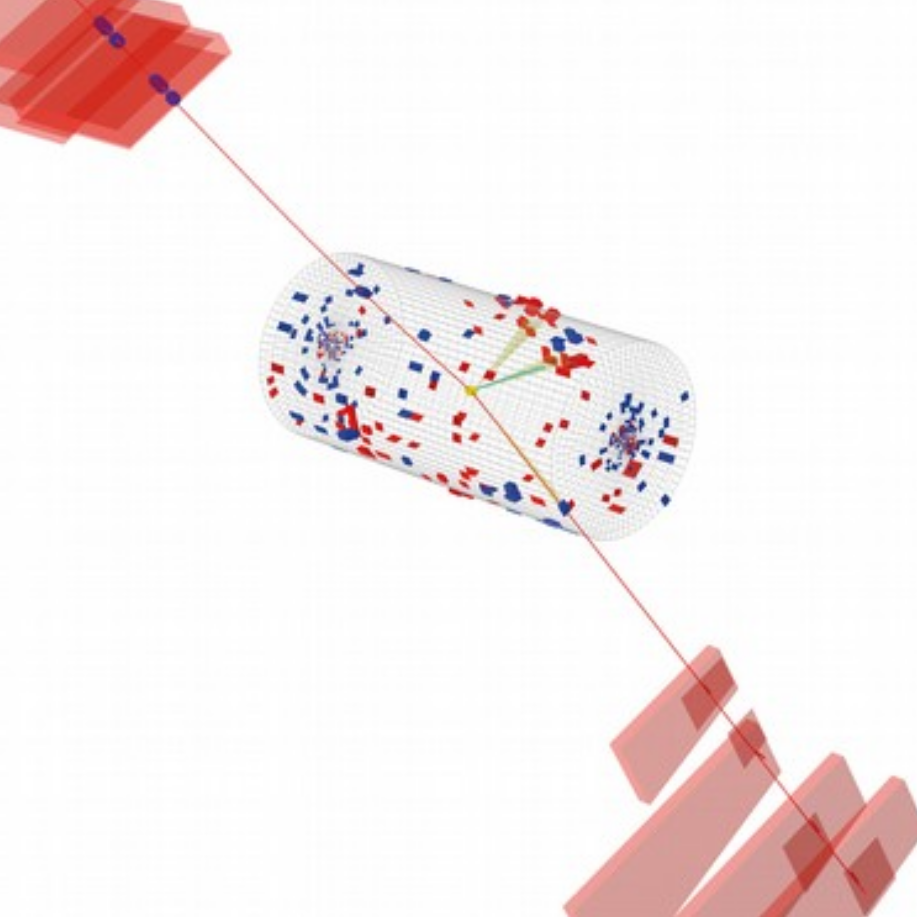
\includegraphics[width=\EmbedPictsWidth cm]{\PhDthesisdir/plots_and_images/from_embedding/Z_to_mumu_data.png}}};
}

\only<2->{
\draw [-latex, very thick] (\EmbedPictsWidth+\EmbedPictsMargin/5, \EmbedPictsWidth/2) -- + (3*\EmbedPictsMargin/5,0);
\draw (\EmbedPictsWidth/2+\EmbedPictsWidth+\EmbedPictsMargin, \EmbedPictsWidth) node [above] {\EmbedPictsTxtSize Remove $\mu\mu$ system};
\node[anchor=south west,inner sep=0] at (\EmbedPictsWidth+\EmbedPictsMargin,0) {\frame{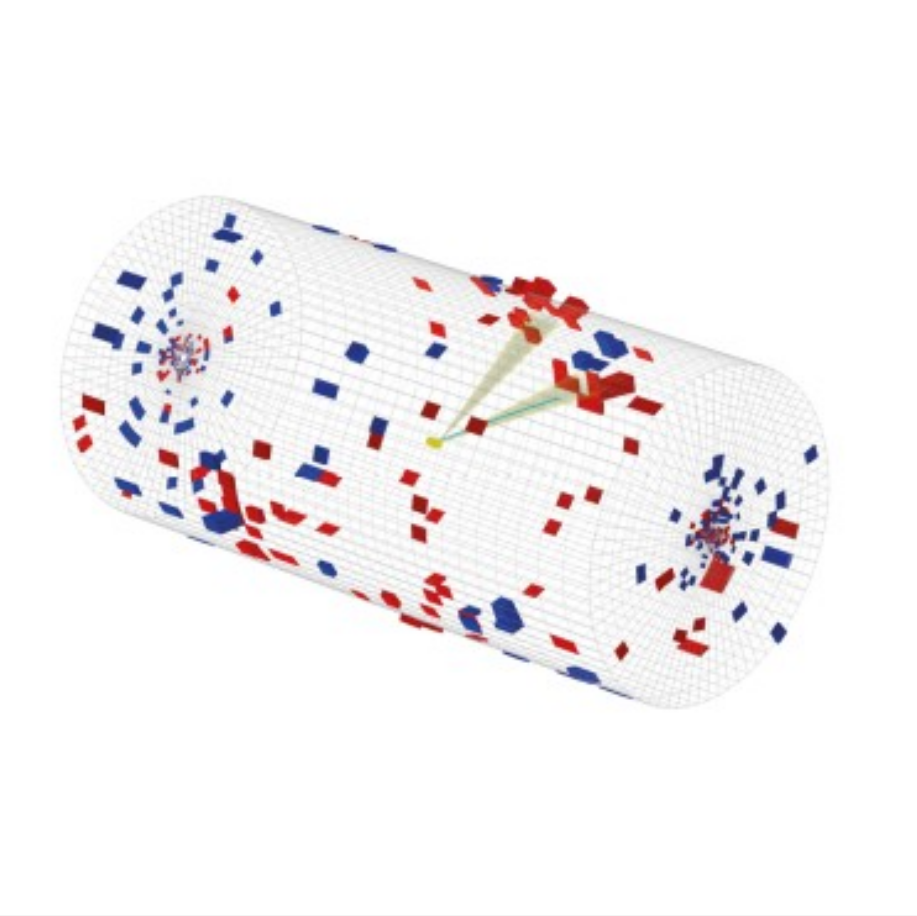
\includegraphics[width=\EmbedPictsWidth cm]{\PhDthesisdir/plots_and_images/from_embedding/remove_mumu.png}}};
}

\only<3->{
\draw (\EmbedPictsWidth+\EmbedPictsMargin,-\EmbedPictsWidth/2-\EmbedPictsMargin) node [above left] {\EmbedPictsTxtSize Simulate $\Zboson\to\tau\tau$};
\draw (\EmbedPictsWidth+\EmbedPictsMargin,-\EmbedPictsWidth/2-\EmbedPictsMargin) node [below left] {\EmbedPictsTxtSize ($\vec{p}_{\tau} \simeq \vec{p}_{\mu}$)};
\node[anchor=south west,inner sep=0] at (\EmbedPictsWidth+\EmbedPictsMargin,-\EmbedPictsWidth-\EmbedPictsMargin) {\frame{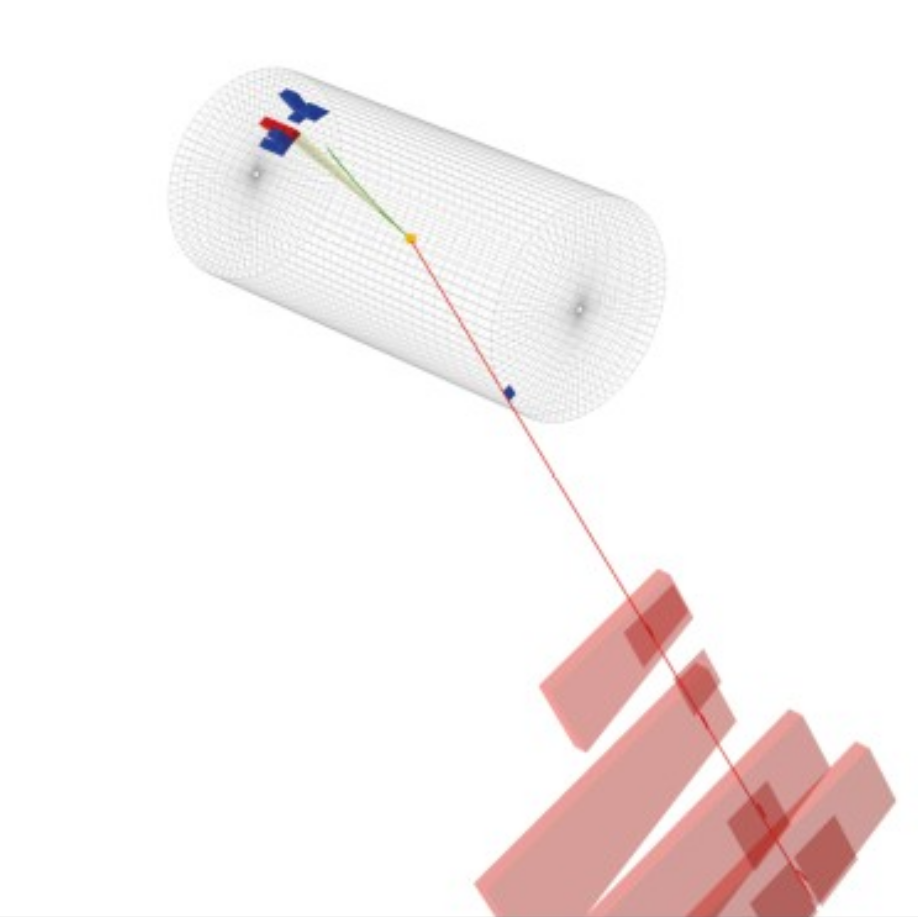
\includegraphics[width=\EmbedPictsWidth cm]{\PhDthesisdir/plots_and_images/from_embedding/Z_to_tautau_simulation.png}}};
}

\only<4->{
\draw [-latex, very thick] (2*\EmbedPictsWidth+6*\EmbedPictsMargin/5, \EmbedPictsWidth/4) -- (2*\EmbedPictsWidth+2*\EmbedPictsMargin-\EmbedPictsMargin/5,0);
\draw [-latex, very thick] (2*\EmbedPictsWidth+6*\EmbedPictsMargin/5,-\EmbedPictsWidth/4-\EmbedPictsMargin) -- (2*\EmbedPictsWidth+2*\EmbedPictsMargin-\EmbedPictsMargin/5,-\EmbedPictsMargin);
\draw (2*\EmbedPictsWidth+2*\EmbedPictsMargin+\EmbedPictsWidth/2,\EmbedPictsWidth/2-\EmbedPictsMargin/2) node [above] {\EmbedPictsTxtSize $\Zboson\to\tau\tau$ embedded event};
\node[anchor=south west,inner sep=0] at (2*\EmbedPictsWidth+2*\EmbedPictsMargin,-\EmbedPictsWidth/2-\EmbedPictsMargin/2) {\frame{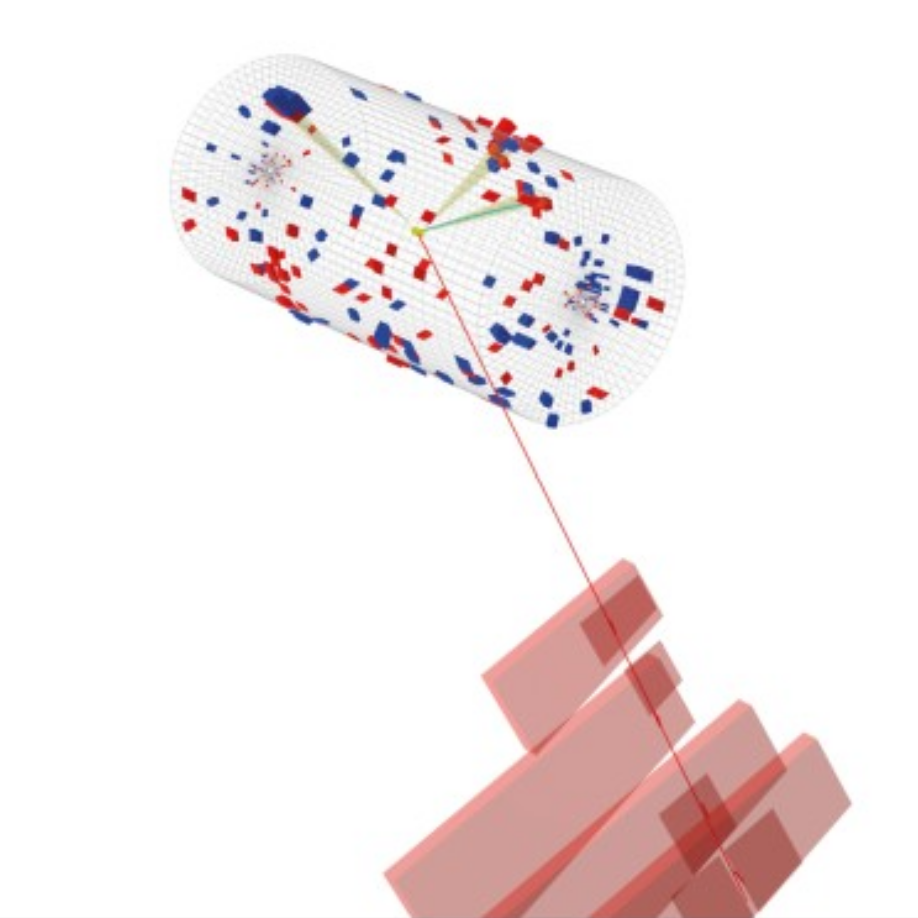
\includegraphics[width=\EmbedPictsWidth cm]{\PhDthesisdir/plots_and_images/from_embedding/embedded_event.png}}};
}

\clip (-1,-\EmbedPictsWidth-\EmbedPictsMargin-.25) rectangle (3*\EmbedPictsWidth+5*\EmbedPictsMargin/2+.25, \EmbedPictsWidth+.5);
\end{tikzpicture}
\end{center}\vspace{-.5\baselineskip}
\end{frame}

\subsection*{Fake \tauh s}
\begin{frame}
\backupslinklabel{ff}
\frametitle{The Fake Factor method \& jets faking \tauh}
\beamercite{CMS-NOTE-2019-170}

\manip How many events contain misidentified \tauh\ (fake taus) in the Signal Region (SR)?

%\pause

\begin{center}
\includegraphics[width=\graphw,height=\graphh/13*10,keepaspectratio]{\PhDthesisdir/plots_and_images/Fake_Factor/FF_ppe-tikz-partial.tex}
\end{center}
\end{frame}

\begin{frame}
\frametitle{Particles isolation -- qualitatively}
\begin{center}
\begin{tikzpicture}
\begin{scope}
\clip (-\graphw/2,-\graphh/2.1) rectangle (\graphw/2,\graphh/2.1);

\drawCMS

\printmuondeposit{7}{10}
\printmuon{7}{10}


\printjetdeposit{9}{-60}
\printmuondeposit{7}{-60}
\printjet{9}{-60}
\printmuonnolabel{7}{-60}

\printtauhdeposit{9}{150}
\printtauh{9}{150}

\printjetdeposit{9}{-150}
\printjetfakenolabel{9}{-150}

\printDR{0.4}{150}
\printDR{0.4}{-150}
\end{scope}

\draw (110:\ECALrout) node [text depth=0pt] (rt) {\textbf{real \tauh:}};
\draw (rt.east) node [right, text depth=0pt] {few tracks = isolated};
\draw (-125:1.1*\Solenrin) node (ft) {\textbf{${\text{jet}\to\tauh}$}};
\draw (ft) node [below] {\textbf{= \ftauh}};
\draw (ft.east) node [below right, text depth=0pt] {more tracks = not isolated};

\draw [ltcolorred, thick, -latex] (rt) to [out = -60, in = 45] (140:.9*\trackerrout);
\draw [ltcolorred, thick, -latex] (ft.east) to [out = 20, in = -50] (-140:.9*\trackerrout);

\end{tikzpicture}
\end{center}
\end{frame}

\begin{frame}
\frametitle{The Fake Factor method: determination regions definitions}
\beamercite{CMS-NOTE-2019-170}

\begin{block}{QCD multijet (\tauh\tauh, \mu\tauh\ and \ele\tauh\ channels)}
Same as SR, except:
\begin{itemize}
\item same signs for $L_1$ and $L_2$ electric charges (opposite signs in the SR).
\end{itemize}
\end{block}

\pause\vfill

\begin{block}{\Wjets\ (\mu\tauh\ and \ele\tauh\ channels)}
Same as SR, except:
\begin{itemize}
\item transverse mass $m_T^{(\ell)}>\SI{70}{\GeV}$ ($m_T^{(\ell)}<\SI{70}{\GeV}$ in the SR);
\item no \quarkb-jet (allowed in the SR).
\end{itemize}
\end{block}

\pause\vfill

\begin{block}{\ttbar\ (\mu\tauh\ and \ele\tauh\ channels)}
Estimation from simulated samples, same selection as in SR.
\end{block}

\vfill
\end{frame}

%\begin{frame}
%\frametitle{The Fake Factor method}
%\beamercite{CMS-NOTE-2019-170}
%
%\manip Maybe the DR are not \SI{100}{\%} pure in terms of process-of-interest.
%
%\manip To ensure purity, slighlty change $\mathrm{FF}_i$ definition
%\begin{equation*}
%\mathrm{FF}_i = \frac{n_\text{iso}}{n_\text{anti-iso}}
%\rightsquigarrow
%\mathrm{FF}_i = \frac{n_\text{iso} - n_\text{iso}^\text{rest}}{n_\text{anti-iso} - n_\text{anti-iso}^\text{rest}}
%\end{equation*}
%\begin{center}
%{\small $n_x^\text{rest}$ = impurity of backgrounds other than from the process-of-interest in the DR, MC-driven.}
%\end{center}
%\end{frame}

\begin{frame}
%\frametitle{The Fake Factor method}
\beamercite{CMS-NOTE-2019-170}
%\vspace{-20pt}
\begin{center}
\includegraphics[width=\graphw,height=\graphh,keepaspectratio]{\PhDthesisdir/plots_and_images/Fake_Factor/FF_ppe-tikz.tex}
\end{center}
\vspace{-4pt}%\vspace{-10pt}
\end{frame}

\subsection*{Discriminating variable}
\begin{frame}
\frametitle{Discriminant variable?}

\vfill

\begin{minipage}[c]{.3\textwidth}
\manip \MET\ due to neutrinos.
\manip No invariant mass!
\end{minipage}
\hfill
\begin{minipage}[c]{.45\textwidth}
\begin{center}
\begin{fmffile}{H-tautau_mutau}\fmfstraight
\begin{fmfchar*}(50,40)
  \fmfleft{h}
  \fmfright{nu1,nub1,tau1,tau2,nub2,nu2}
  \fmf{dashes, label=$\Hs,, \Hn,, \Ha$, l.side=left, tension=5}{h,v}
  \fmf{fermion, label=$\antitau$, l.side=left, tension=4}{t1d,v}
  \fmf{fermion, label=$\leptau$, l.side=left, tension=4}{v,t2d}
  \fmf{fermion, tension=3}{nu1,t1d}
  \fmf{boson, label=$\Wbosonplus$, l.side=left, tension=2}{t1d,W1d}
  \fmf{fermion}{tau1,W1d,nub1}
  \fmf{fermion, tension=3}{t2d,nu2}
  \fmf{boson, label=$\Wbosonminus$, tension=2}{t2d,W2d}
  \fmf{fermion}{tau2,W2d,nub2}
  \fmflabel{$\antinutau$}{nu1}
  \fmflabel{$\nutau$}{nu2}
  \fmflabel{$\antinumu$}{nub2}
  \fmflabel{$\muon$}{tau2}
  \fmflabel{$\antiquark$}{tau1}
  \fmflabel{$\quark$}{nub1}
  \fmfdot{v,t1d,t2d,W1d,W2d}
\end{fmfchar*}
\end{fmffile}

\end{center}
\end{minipage}
\hfill~

\vfill\pause

\begin{minipage}[c]{.55\textwidth}
\manip For muon and \MET,
\begin{equation*}
\mT(\mu,\MET) = \sqrt{2p_T^{(\mu)} \MET (1-\cos\Delta\phi)}
\end{equation*}
\begin{center}
\begin{tikzpicture}
\def\aangle{30}
\def\bangle{150}
\def\aRadius{1.75}
\def\bRadius{1.25}
\def\cRadius{.5}
\draw [-latex, ltcolorred] (0,0) --+ (\aangle:\aRadius) node [above] {$\vpT^{(\mu)}$};
\draw [-latex, ltcolorblue] (0,0) --+ (\bangle:\bRadius) node [above] {$\vMET$};
\draw (\aangle:\cRadius) arc (\aangle:{(\aangle+\bangle)/2}:\cRadius) node [above] {$\Delta\phi$}  arc ({(\aangle+\bangle)/2}:\bangle:\cRadius);
\end{tikzpicture}
\end{center}
\end{minipage}
\qquad
\begin{minipage}[c]{.35\textwidth}
\begin{center}
\begin{fmffile}{qq_W_mu_nu}%\fmfstraight
\begin{fmfchar*}(30,15)
  \fmfleft{q1,q2}
  \fmfright{l1,l2}
  \fmf{fermion}{q1,v1,q2}
  \fmf{boson, label=$\Wbosonminus$}{v1,v2}
  \fmf{fermion}{l2,v2,l1}
  \fmflabel{$\quarkd$}{q1}
  \fmflabel{$\antiquarku$}{q2}
  \fmflabel{$\muon$}{l1}
  \fmflabel{$\antinumu$}{l2}
  \fmfdot{v1,v2}
\end{fmfchar*}
\end{fmffile}

\end{center}
\end{minipage}
\hfill

\vfill 

\end{frame}

\begin{frame}
\frametitle{Discriminant variable: \mTtot}
\manip For $L_1$, $L_2$ and \MET\ system,
\begin{equation*}
\boxed{\mTtot = \sqrt{\mT^2(L_1,\MET) + \mT^2(L_2,\MET) + \mT^2(L_1,L_2)}}
\end{equation*}
\begin{minipage}[c]{.6\textwidth}
\begin{equation*}
\mT(1,2) = \sqrt{2p_T^{(1)} p_T^{(2)} (1-\cos\Delta\phi)}
\end{equation*}
\end{minipage}
\begin{minipage}[c]{.35\textwidth}
\begin{center}
\begin{tikzpicture}
\def\aangle{30}
\def\bangle{150}
\def\aRadius{1.75}
\def\bRadius{1.25}
\def\cRadius{.5}
\draw [-latex, ltcolorred] (0,0) --+ (\aangle:\aRadius) node [above] {$\vpT^{(1)}$};
\draw [-latex, ltcolorblue] (0,0) --+ (\bangle:\bRadius) node [above] {$\vpT^{(2)}$};
\draw (\aangle:\cRadius) arc (\aangle:{(\aangle+\bangle)/2}:\cRadius) node [above] {$\Delta\phi$}  arc ({(\aangle+\bangle)/2}:\bangle:\cRadius);
\end{tikzpicture}
\end{center}
\end{minipage}
\end{frame}


\subsection*{Results}

\begin{frame}
\begin{center}
\LARGE Results obtained in this thesis?
\end{center}
\end{frame}

\begin{frame}
\frametitle{\mTtot\ distributions}

\begin{minipage}[t]{.49\textwidth}

\manip Backgrounds = SM expectations:
\submanip DY $\Zboson\to\tau\tau$ and some \ttbar\ in \colorbox{\EMBcolor}{$\mu\to\tau$ embedded}
\submanip QCD, \Wjets\ and some \ttbar\ in \colorbox{\FAKEScolor}{$\text{Jet}\to\tauh$}
\submanip $\Zboson\to\ele\ele$ + $\Zboson\to\mu\mu$ in \colorbox{\ZLLcolor}{$\Zboson\to\ell\ell$}
\submanip Remaining \ttbar\ in \colorbox{\TTBARcolor}{\ttbar}
\submanip Other small backgrounds in \colorbox{\DIBcolor}{Diboson}

\only<2->{\manip \Higgs\ at \SI{400}{\GeV} expected $\sigma\times\BR=\SI{1}{\pico\barn}$ \tikzmarknode{signal.}{nodesignal}}

\only<3->{\manip Compare to observed events (black dots).}

%\vspace{\baselineskip}
%
%\manip Lots of work to obtain this!
%\submanip simulated events
%\submanip detector issues
%\submanip uncertainties measured
%\manip Collaboration with KIT (Germany)
%
%\vspace{\baselineskip}

\only<4->{\manip Data/Bkg agreement $\to$ \textbf{exclusion limits} on $\sigma\times\BR$}
\end{minipage}
\hfill
\begin{minipage}[t]{.49\textwidth}
\begin{center}
\vspace{-2\baselineskip}

%\only<1>{\plotHTTshapes{mt_tot}{mssm_classic}{2018}{tt}{32}{prefit_nosignal_blinded}}
\only<1-2>{\plotHTTshapes{mt_tot}{mssm_classic}{2018}{tt}{32}{prefit_blinded}}
\only<3->{\plotHTTshapes{mt_tot}{mssm_classic}{2018}{tt}{32}{prefit}}
\end{center}
\end{minipage}

\begin{tikzpicture}[overlay, remember picture]
\only<2>{
\draw [ltcolorred, very thick, -latex] (nodesignal) to [out=0, in=-165] (11.45,5);
}
\only<5>{
\fill [white, opacity=.9] (0,0) rectangle (.5\textwidth, .85\textheight);
\draw (.025\textwidth, .7\textheight) node [right, text depth=0pt] (A) {\manip \textbf{Lot} of hard work to obtain this:};
\draw (A.north) node [above] {\textbf{Not \emph{just} a plot!}};

\foreach \txt in {simulated events, detector issues, uncertainties measured}{
\draw (A.south west) node [below right] (A) {\submanip \txt};
}
\draw (A.south west) node [below right] (A) {\manip Collaborative work:};
\foreach \txt in {Karlsruhe Institute of Technology (DE), Imperial College (UK), DESY (DE), HEPHY (AT), IP2I (FR)}{
\draw (A.south west) node [below right] (A) {\submanip \txt};
}
}
\end{tikzpicture}
\end{frame}

\begin{frame}
%\frametitle{Exclusion limits}
\beamercite{CLs_method}

\begin{minipage}[c]{.49\textwidth}
\begin{center}
\only<1-5>{\plotHTTModelIndepLimits{mssm_classic}{combined}{ggH}{_cmb}}
\only<6->{\plotHTTModelIndepLimits{mssm_classic}{combined}{ggH}{_cmb_vs_CMS_ATLAS}}
\end{center}
\end{minipage}
\hfill
\begin{minipage}[c]{.49\textwidth}
\only<2-5>{\begin{center}
\plotHTTshapes{mt_tot}{mssm_classic}{2018}{tt}{32}{prefit}
\end{center}}
\only<6->{
\manip CMS 2016:
\beamerlocalcite{CMS-PAS-HIG-17-020}
\manip ATLAS Run~II:
\beamerlocalcite{ATLAS-MSSM-HTT_2020}
}
\end{minipage}

\begin{tikzpicture}[overlay, remember picture]
\only<2-4>{
\draw [ltcolorred, very thick] (.935\textwidth, .5\textheight) circle (.4) ;
\draw [ltcolorred, thick, dotted] (3.56,1) --+ (0, 3.9);
}

\only<3-4>{
\draw [ltcolorred, very thick, latex-] (11.45, 4.8) --+ (0, -.4);
\draw [ltcolorred, very thick, latex-] (11.45, 5.1) --+ (0, .4) node [above] {\small $\sigma\times\BR=\SI{1}{\pico\barn}$};
}

\only<4>{
\def\ypos{4.28}
\draw [ltcolorred, thick, dotted] (1.3, \ypos) --+ (6,0);
\draw [ltcolorred, very thick] (11.45,4.95) ellipse (.3 and .6) ;
\fill [ltcolororange] (3.56,\ypos) circle (3pt) ;
\draw [ltcolorred, very thick, -latex] (11.15,4.95) to [out=-180, in = 0] (3.56,\ypos) ;
}

\only<5>{
\draw [ltcolorred] (3.56,4) node [right] {Would have been seen} ;
\draw [ltcolorred] (3.56,2) node [left] {Can't tell} ;
}
\end{tikzpicture}
\end{frame}

\begin{frame}
%\frametitle{Model-dependant limits}

\begin{minipage}[c]{.49\textwidth}
\only<1>{\manip Model dependent limits:
\submanip Fix high-order MSSM parameter,
\submanip Explore $(m_{\HiggsA},\tan\beta)$ plane,
\submanip Do data stick more to SM or MSSM?}
\only<2->{
\begin{center}
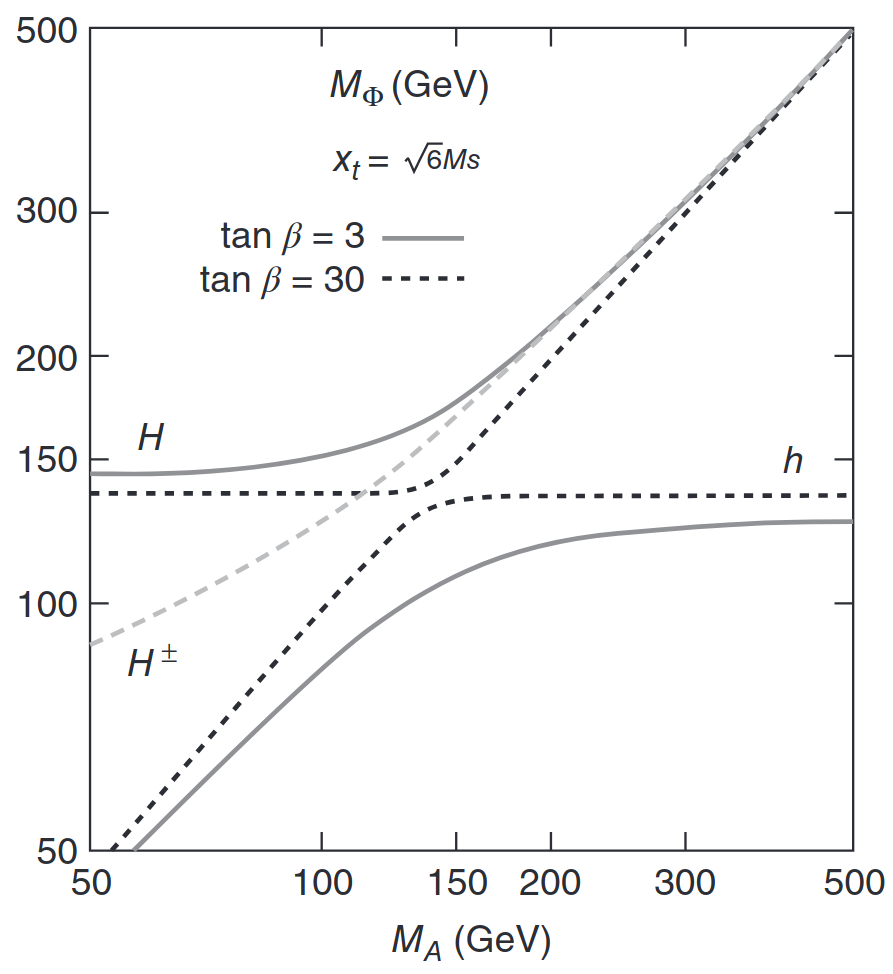
\includegraphics[height=\graphh]{\PhDthesisdir/plots_and_images/from_Nagashima_BSM/fig_1-9.tex}
\end{center}
}
\end{minipage}
\hfill
\begin{minipage}[c]{.49\textwidth}
\begin{center}
\plotHTTModelDepLimits{mssm_vs_sm_h125}{_vs_CMS}
\end{center}
\end{minipage}

\begin{tikzpicture}[overlay, remember picture]
\draw [ltcolorred] (10.5,4) node {data = more SM-like} ;
\draw [ltcolorred] (14,2.5) node {Can't tell} ;

\only<2->{
\draw [ltcolororange, ultra thick] (12.5, 1) ellipse (2.5 and .5);
\draw [ltcolororange, ultra thick] (5.5, 3.6) ellipse (2 and .5);
}
\end{tikzpicture}

\end{frame}